\documentclass{beamer}
%
% Choose how your presentation looks.
%
% For more themes, color themes and font themes, see:
% http://deic.uab.es/~iblanes/beamer_gallery/index_by_theme.html
%
\mode<presentation>
{
  \usetheme{default}      % or try Darmstadt, Madrid, Warsaw, ...
  \usecolortheme{default} % or try albatross, beaver, crane, ...
  \usefonttheme{default}  % or try serif, structurebold, ...
  \setbeamertemplate{navigation symbols}{}
  \setbeamertemplate{caption}[numbered]
} 

\usepackage[english]{babel}
\usepackage[utf8x]{inputenc}

\usepackage{graphicx}
\usepackage{subcaption}

\usepackage{amsthm}
\usepackage{amsmath}
\usepackage{amssymb}

\usepackage{mathrsfs}

\DeclareMathOperator*{\argmin}{arg\,min}
\DeclareMathOperator*{\argmax}{arg\,max}

\renewcommand{\vec}[1]{\mathbf{#1}}

\usepackage{hhline}
\usepackage{makecell}

\usepackage[width=\textwidth]{caption}
\usepackage{float}

\usepackage[linesnumbered, ruled, vlined]{algorithm2e}
\SetKwRepeat{Do}{do}{while}
\SetKwProg{Fn}{Function}{}{}

\newcommand{\codef}[1]{code_{CT}(#1)}
\newcommand{\codest}[1]{code_{ST}(#1)}
\newcommand{\codeset}{\mathcal{C}}
\newcommand{\codetable}{CT}
\newcommand{\codetables}{\mathcal{CT}}
\newcommand{\codingset}{CS}
\newcommand{\cover}[2]{cover(#1,#2)}

\newcommand{\dataset}{\mathcal{D}}
\newcommand{\fset}{\mathscr{F}}
\newcommand{\groei}{\texttt{Groei}}
\newcommand{\groeinos}{\texttt{GroeiNoS}}
\newcommand{\slim}{\texttt{Slim}}
\newcommand{\itemset}{\mathcal{I}}
\newcommand{\krimp}{\texttt{Krimp}}
\newcommand{\lossf}{\mathcal{L}}

\newcommand{\model}{H}
\newcommand{\modelset}{\mathcal{H}}

\newcommand{\natnumbers}{\mathbb{N}}
\newcommand{\prob}{\mathbb{P}}

\newcommand{\setitemsets}{\mathcal{F}}
\newcommand{\standardtable}{ST}
\newcommand{\structuref}[1]{\mathcal{K}_{#1}}

\newcommand{\transaction}{t}
\newcommand{\usage}[1]{usage_\dataset(#1)}

\newcommand{\bigonot}{\mathcal{O}}

\title[Ensemble of Code Tables]{Ensemble of Code Tables \\ (Master Thesis Defense)}
\author{Jaspreet Singh}
\institute{Utrecht University}
\date{July 10th 2018}

\begin{document}

\begin{frame}
  \titlepage
\end{frame}

\begin{frame}{Outline}
 \tableofcontents
\end{frame}

\section{Introduction}

\begin{frame}{Introduction: Machine Learning Models}
\begin{itemize}
  \item \textbf{Goal}: Give a description of the database by using some model
  \item \ldots by approximating the underlying data distribution.
  \item \textit{Example}: Find interesting patterns in the data. 
  \item \textit{Example}: Find groups of transactions that are similar.
  \item \textit{Example}: Detect anomalies in the data.
\end{itemize}
\end{frame}

\begin{frame}{Introduction}
\begin{itemize}
  \item \textbf{Goal}: \textit{Cluster} the data such that \textit{overlap} is allowed between the clusters.
  \item \textbf{How}: Use a \textit{series of code tables}, such that each code table captures \textit{a certain aspect} of the data.
\end{itemize}
\end{frame}

\begin{frame}{Introduction: Clustering}
\begin{itemize}
  \item A group of data points which are similar in some sense.
  \item Is an unsupervised machine learning method.
  \item Performed in exploratory data analysis.
  \item Different types of clustering methods:
\end{itemize}

\begin{figure}
  \centering
  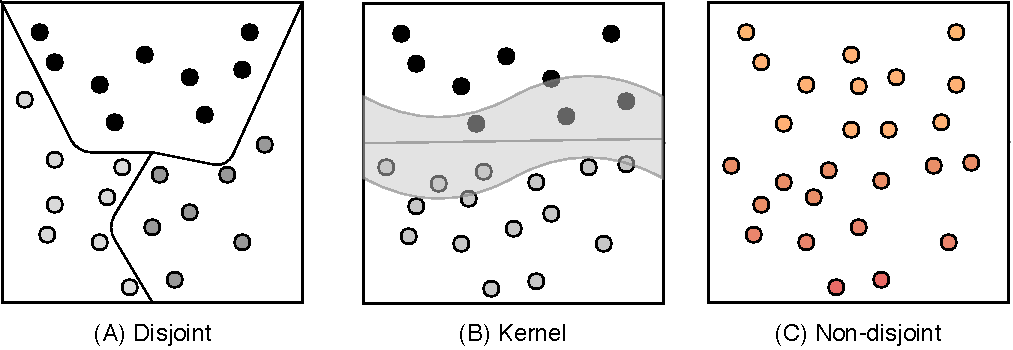
\includegraphics[width=\textwidth]{img/clusterTypes}
  \label{fig:clusterTypes}
\end{figure}

\end{frame}

\begin{frame}{Introduction: Code Tables}
\begin{itemize}
  \item A code table is used to encode (compress) all the transactions in a dataset. 
  \item A code table alone is not very useful, an algorithm which uses a code table is required.
  \item This algorithm is called the \texttt{Cover} algorithm
\end{itemize}
\end{frame}

\begin{frame}{Introduction: Code Tables}
\begin{figure}
  \centering
  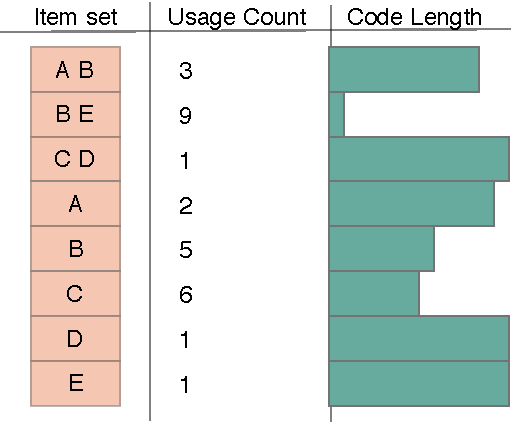
\includegraphics[width=\textwidth]{img/CodeTableExample}
  \label{fig:CodeTableExample}
\end{figure}
\end{frame}

\begin{frame}{Introduction: Code Tables}
\begin{figure}
  \centering
  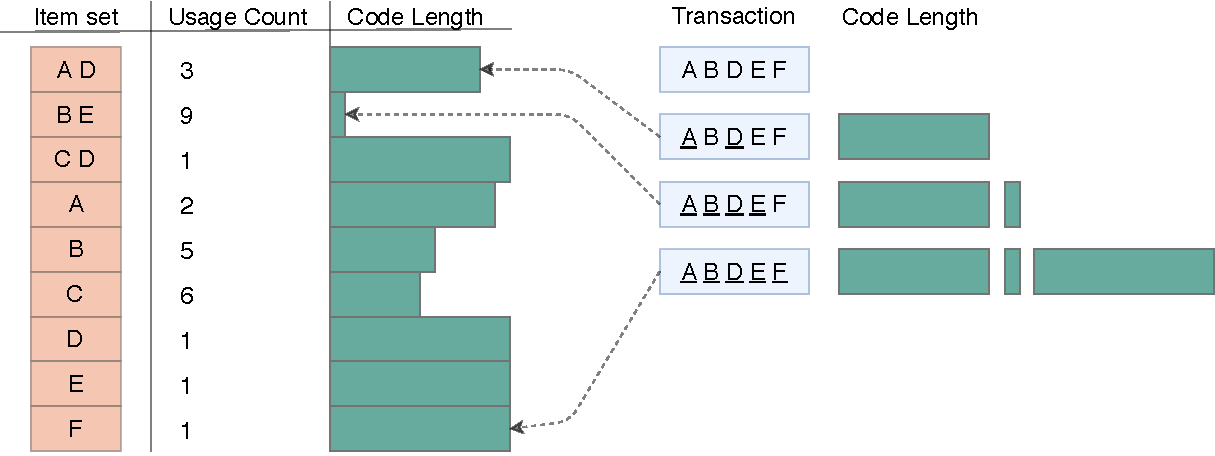
\includegraphics[width=\textwidth]{img/CodeTableExample2}
  \label{fig:CodeTableExample2}
\end{figure}
\end{frame}

\section{Preliminaries}
\begin{frame}{Preliminaries}
\begin{itemize}
	\item Basic Definitions
	\item Minimum Description Length Principle (MDL)
	\item Compression and Machine Learning
	\item Clustering
	%\item Ensemble Structures
\end{itemize}
\end{frame}

\begin{frame}{Preliminaries: Basic Definitions}
\begin{itemize}
	\item A dataset $\dataset$ is represented as a $N\times M$ binary matrix. 
	\item $N$ denotes the number of rows (transactions).
	\item $M$ denotes the number of columns (items).
	\item $(t, i) = 1$ denotes that item $i$ is used in transaction $t$.
	\item The set of items $\itemset$ make up the `alphabet' of the dataset.
	\item An itemset $I$ is an element of $\mathcal{P}(\itemset)$: $I \in \mathcal{P}(\itemset)$.
\end{itemize}
\end{frame}

\begin{frame}{Preliminaries: Basic Definitions}
\begin{itemize}
	\item The support of an itemset $supp_\dataset (I)$, is the number of transactions in which $I$ occurs:
	\[supp_\dataset (I) = |\{t \in \dataset \mid I \subseteq t\}|\]
	\item Itemsets are frequent with respect to some minimum support $\theta$.
	\item This restricts the number of possible itemsets.
	\item Given a minimum support $\theta$, the set of all frequent itemsets $\setitemsets$ is defined as:
	\[\{I \in \setitemsets \mid supp_\dataset (I) \geq \theta\}\]
\end{itemize}
\end{frame}


\begin{frame}{Preliminaries: Minimum Description Length Principle}
Given a set of models $\modelset$, the best model $\model \in \modelset$ is the model that minimises \[L(H) + L(\dataset \mid \model)\]
\begin{itemize}
	\item $L(\model)$ is the length of the description of $\model$ in bits.
	\item $L(\dataset\mid\model)$ is the length of the description of the data in bits, encoded by using $\model$.
\end{itemize}
\end{frame}

\begin{frame}{Preliminaries: Minimum Description Length Principle}
\begin{itemize}
	\item MDL is a practical version of the Kolmogorov Complexity.
	\item The Kolmogorov Complexity cannot be computed. 
	\item The Kolmogorov Complexity of an object is the length of the shortest program that produces the object as output. 
	\item \textit{Example}: The string `abababab' can be described as: $4 \times$ `ab'
\end{itemize}
\end{frame}


% CT AND KRIMP
\begin{frame}{Preliminaries: Compression and Machine Learning}
MDL applied to item sets: Code Tables!
\begin{itemize}
	\item Use item sets to describe the data through code tables
\end{itemize}

\begin{block}{Definition: Code Table}
Let $\itemset$ be a set of items and $\codeset$ be a set of codes. A code table $\codetable$ over $\itemset$ and $\codeset$ is a table with two columns such that: The first column contains subsets over $\itemset$, all singleton item sets must be present. The second column contains codes from $\codeset$ and every code is allowed to occur at most once.
\end{block}

\begin{itemize}
	\item The standard code table $\codetable_{ST}$ only contains the singleton item sets.
\end{itemize}
\end{frame}

%Cover
\begin{frame}{Preliminaries: Compression and Machine Learning}
\begin{figure}[H]
  \centering
   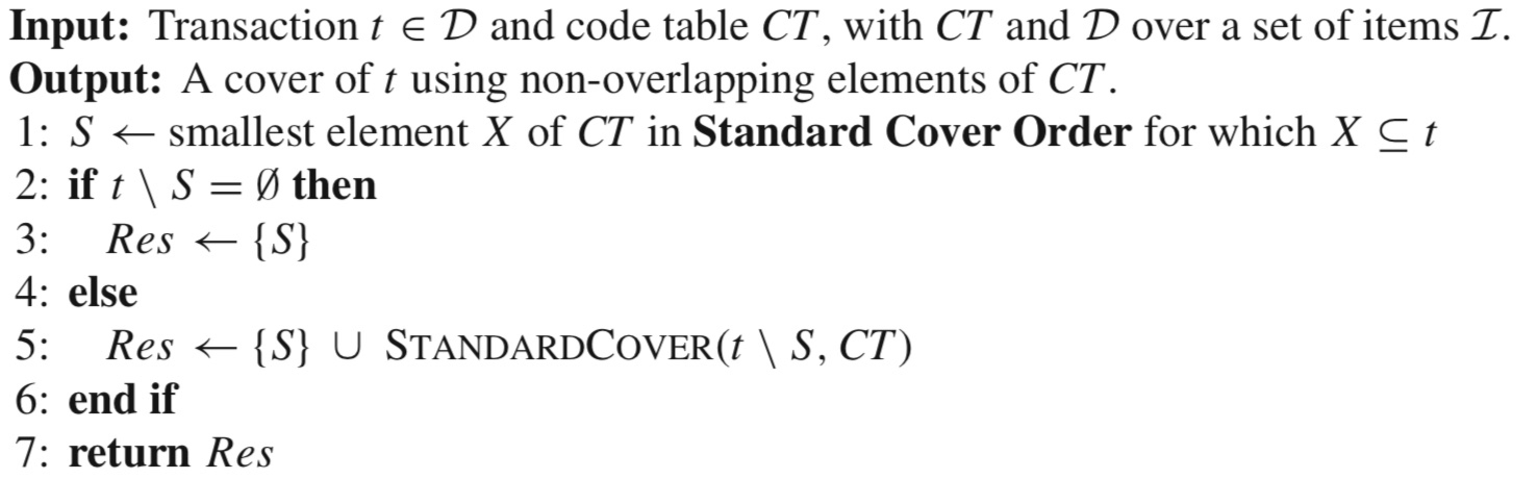
\includegraphics[width=\textwidth]{img/cover}
\end{figure}
\end{frame}

\begin{frame}{Preliminaries: Compression and Machine Learning}
\begin{itemize}
	\item The item sets in the code tables are sorted to avoid trying all combinations to cover a transaction
	\item The sorting order is called: \textbf{Standard Cover Order}
			\begin{enumerate}
				\item Sort descending on item set size $|I|$
				\item Sort descending on support
				\item Sort ascending lexicographically
			\end{enumerate}
\end{itemize}
\end{frame}

\begin{frame}{Preliminaries: Compression and Machine Learning}
\begin{itemize}
	\item Actual codes are not needed, code lengths are used to compute the compressed size.
	\item The more an item set is used, the shorter its code length is.
	\item The usage count of an item set $I$ is \[usage(I) = |\{t \in \dataset \mid I \in cover(\codetable, t)\}|\]
	\item This implies a probability distribution of $I \in \codetable$ \[\prob(I \mid \dataset) = \frac{usage(I)}{\sum_{Y\in\codetable}usage(Y)}\]
	\item The code length $L(code_{\codetable}(I))$ then is \[L(code_{\codetable}(I)) = -log(\prob(I\mid\dataset))\]
\end{itemize}
\end{frame}

\begin{frame}{Preliminaries: Compression and Machine Learning}
\begin{block}{Lemma 1}
For any $t\in\dataset$ its encoded size in bits $L(t \mid \codetable)$ is:
\[L(t \mid \codetable) = \sum\limits_{I\in cover(\codetable,t)} L(code_{\codetable}(I))\]
The encoded size of $\dataset$ when encoded by $\codetable$, $L(\dataset \mid \codetable)$, is:
\[L(\dataset\mid\codetable) = \sum\limits_{t\in\dataset} L(t\mid\codetable)\]
The length of a code table $L(\codetable \mid \dataset)$ is:
\[L(\codetable \mid \dataset) = \sum\limits_{I \in \codetable} L(code_{ST}(I)) + L(code_{\codetable}(I))\]
The total encoded length $L(\dataset, \codetable)$ then is:
\[L(\dataset, \codetable) = L(\dataset \mid \codetable) +  L(\codetable \mid \dataset)\]

\end{block}
\end{frame}

\begin{frame}{Preliminaries: Compression and Machine Learning: \texttt{Krimp}}
\begin{itemize}
	\item Many algorithms use a pre-mined set of candidate item sets $\setitemsets$.
	\item $\setitemsets$ is traversed in \textbf{Standard Candidate Order}
			\begin{enumerate}
				\item Sort descending on support
				\item Sort descending on item set size $|I|$
				\item Sort ascending lexicographically
			\end{enumerate}
\end{itemize}
\end{frame}

\begin{frame}{Preliminaries: Compression and Machine Learning: \texttt{Krimp}}
\begin{figure}[H]
  \centering
   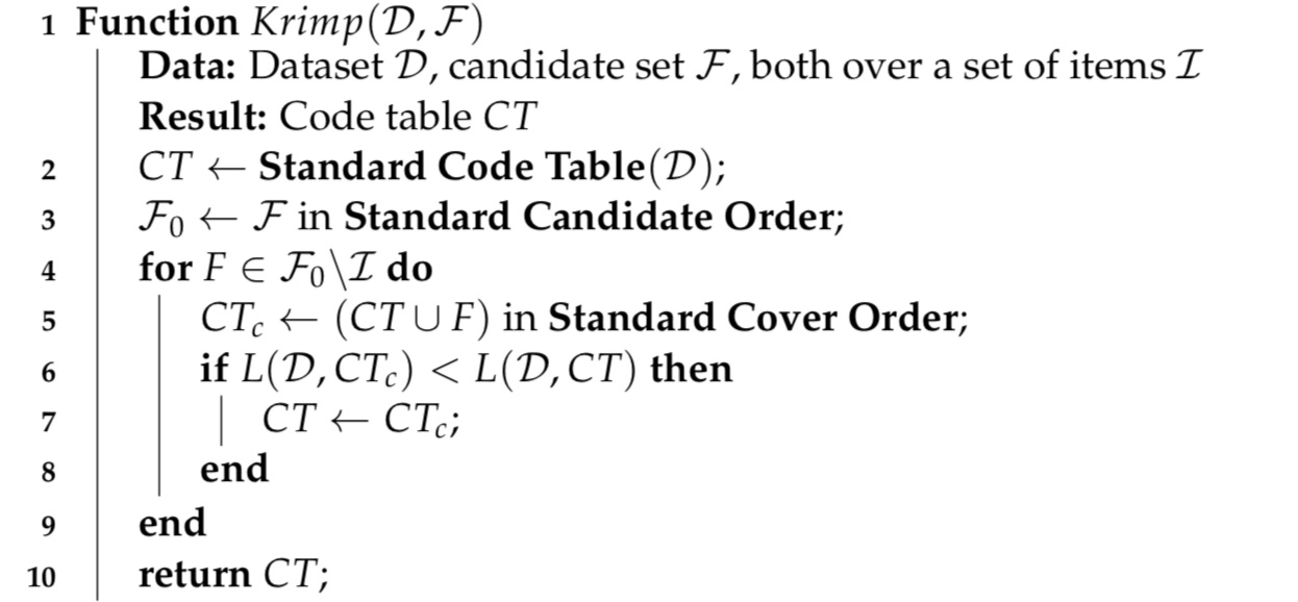
\includegraphics[width=\textwidth]{img/krimp}
\end{figure}
\end{frame}

% SLIM
\begin{frame}{Preliminaries: Compression and Machine Learning: \texttt{Slim}}
\begin{itemize}
	\item Mining a set of (frequent) item sets can take a lot of time.
	\item When dropping the the minimum support $\theta$, the number of frequent item sets explode.
	\item It is possible to generate candidates more efficiently!
	\item \textbf{Insight}: Every item set is the union of two other item sets.
	\item Generate candidate item sets directly from code tables.
\end{itemize}
\end{frame}

\begin{frame}{Preliminaries: Compression and Machine Learning: \texttt{Slim}}
\begin{figure}[H]
  \centering
   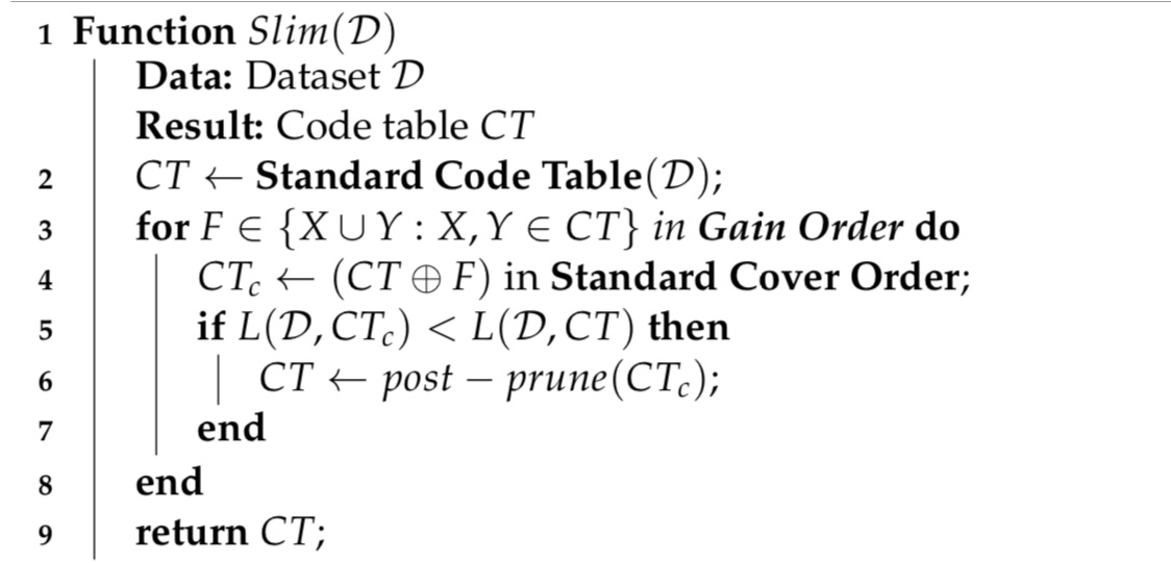
\includegraphics[width=\textwidth]{img/slim}
\end{figure}
\end{frame}

% GROEI
\begin{frame}{Preliminaries: Compression and Machine Learning: \groei}
\begin{itemize}
	\item Use a number of code tables to gain insight in the data from different aspects.
	\item All output code tables contain the same number of non-singleton item sets.
	\item This produces a structure function $\kappa_\dataset$
	\item Allows for the study of the correlation structure at different levels of granularity.
\end{itemize}
\end{frame}

\begin{frame}{Preliminaries: Compression and Machine Learning: \groei}
\begin{figure}[H]
  \centering
   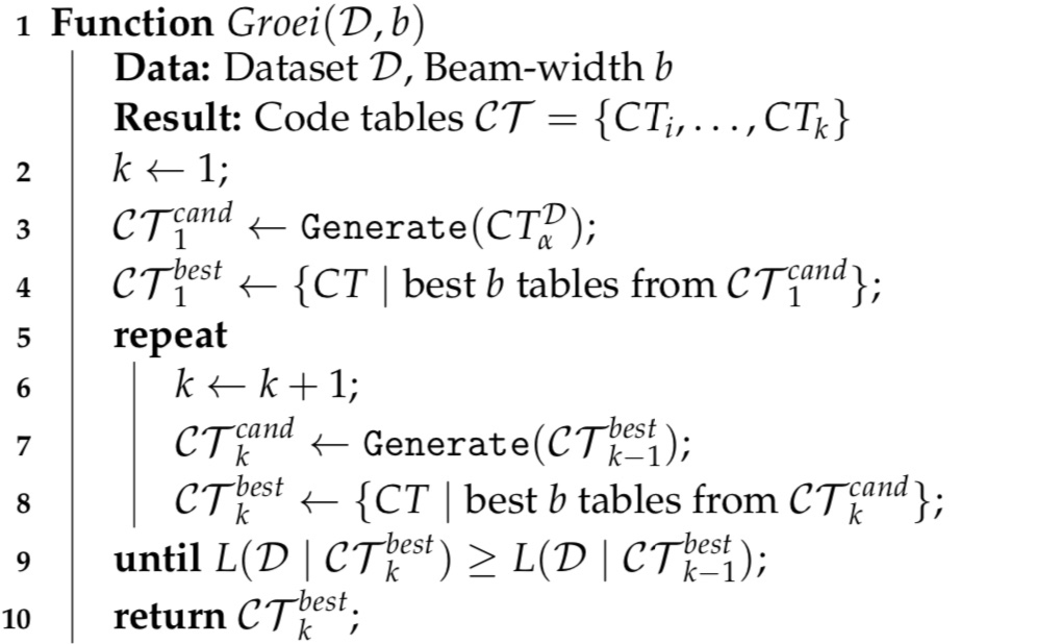
\includegraphics[width=\textwidth]{img/groei}
\end{figure}
\end{frame}

\begin{frame}{Preliminaries: Summary}
\begin{itemize}
	\item The \texttt{Cover} algorithm allows to compress the data by using code tables.
	\item \texttt{Krimp} uses a pre-mined set of item sets.
	\item The number of candidates explodes when the minimum support is lowered.
	\item \texttt{Slim} avoids this explosion by directly generating candidates from the code table.
	\item \texttt{Groei} outputs a number of code tables which together produce a structure function.
\end{itemize}
\end{frame}


% CLUSTERING
\begin{frame}{Preliminaries: Clustering: Hard}
Let $\dataset$ denote the dataset, $K$ the number of clusters and $\dataset_i \subseteq \dataset$ a cluster. A hard partitioning of data set $\dataset$ tries to find $K$ partitions such that:
	\begin{enumerate}
		\item $\forall i \in [1,K]: \dataset_j \neq \emptyset$ \\ All partitions must be non-empty.
		\item $\bigcup\limits_{i=1}^{K} \dataset_i = \dataset$ \\ All partitions together must contain all transactions.
		\item $\forall i,j \in [1,K]: i \neq j \Rightarrow \dataset_i \cap \dataset_j = \emptyset$ \\ There is no overlap between the partitions.
	\end{enumerate}
\end{frame}

\section{Problem Description and Research Questions}
\begin{frame}{Problem Description and Research Questions}
	\begin{itemize}
		\item Observations and Definitions
		\item Problem Description
		\item Research Questions
	\end{itemize}
\end{frame}

\begin{frame}{Problem Description: Observations}
\begin{itemize}
	\item \groei\ produces a number of code tables.
	\item However, all code tables are of the same complexity and are not the best compressing tables.
	\item Get rid of the structure function and make candidate generation more efficient.
	\item We do not want a disjoint clustering, a non-disjoint clustering is required.
	\item Each code table corresponds to a cluster.
	\item It is also possible for a transaction to belong to all clusters with a degree of membership $u_{i,j} \in [0,1]$,the membership coefficient of the $j$th object in the $i$th cluster. 
	\item The membership coefficient must satisfy the following two constraints: \[\forall j: \sum\limits_{i=1}^{K} u_{i,j} = 1 \qquad\text{and}\qquad \forall i: \sum\limits_{j=1}^{N} u_{i,j} < N\]

\end{itemize}
\end{frame}

\begin{frame}{Problem Description: Definitions}
The Membership Coefficient is the probability that tuple $d_j \in \dataset$ belongs to cluster $C_i$: \[\prob(d_j \in C_i) = \frac{2^{-\codetable_i(d_j)}}{\sum\limits_l^C 2^{-\codetable_l(d_j)}}\]

The Encoded Cluster Length of a cluster $C_i$ is determined by its code table $\codetable_i$, and is the Code Table Encoded Length over all the transactions in the database $\dataset$:
\[L(C_i \mid \codetable_i) = \sum\limits_{j=1}^{N} L(d_j \mid \codetable_i)\]
\end{frame}

\begin{frame}{Problem Description}
Let $\dataset$ denote a database, and let $\itemset$ denote the set of items in the database. The database $\dataset$ is then a subset of $\mathcal{P}(\itemset)$, $\dataset \subseteq \mathcal{P}(\itemset)$. So, every tuple $t \in \dataset$ is also an element of $\mathcal{P}(\itemset)$. The goal is then to find the code table $\codetable$ that best compresses $\dataset$.
\[
	\min \codetable(\dataset)
\]
\end{frame}

\begin{frame}{Problem Description}
Let $\dataset$ denote a database, and let $\codetables$ denote a set of code tables such that $\codetable_1, \codetable_2 \in \codetables$. Then either:
\begin{itemize}
	\item $\codetable_1, \codetable_2 \in \codetables$ form an antichain;
	\item or, $\exists \dataset_1, \dataset_2 \subset \dataset$ given both partitions are large enough that: \[\codetable_1(\dataset_1) \leq \codetable_1(\dataset_2) \qquad\text{and}\qquad \codetable_2(\dataset_2) \leq \codetable_2(\dataset_1)\]
\end{itemize}
\end{frame}

\begin{frame}{Problem Description}
let $\dataset$ denote a database, let $\codetables$ denote a set of code tables, let $Q$ denote some quality threshold, and let $C$ denote the number of code tables possible for $\dataset$ 
\[\forall i \in [1,C]: \big[\codetable_i(\dataset) > Q \Rightarrow  \codetable_i \notin \codetables \big]\]
\end{frame}

\begin{frame}{Research Questions}
\begin{itemize}
	\item Do the obtained clusters capture the characteristics of the underlying data distribution?
	\item Are the clusters dissimilar enough to each describe a specific characteristic of the database?
	\item Are the obtained clusters able to identify a multi-valued relationship, if present? 
	\item Is the runtime low enough for interactive usage?
\end{itemize}
\end{frame}

\section{Algorithms}

\begin{frame}{Clustering Algorithms}
	\begin{itemize}
		\item \texttt{GroeiNoS}
		\item Candidate Generation
		\item \texttt{Slim} Candidate Generation (\texttt{GroeiSlimNoS})
	\end{itemize}
\end{frame}

\begin{frame}{Clustering Algorithms: \groeinos}
\begin{figure}[H]
  \centering
   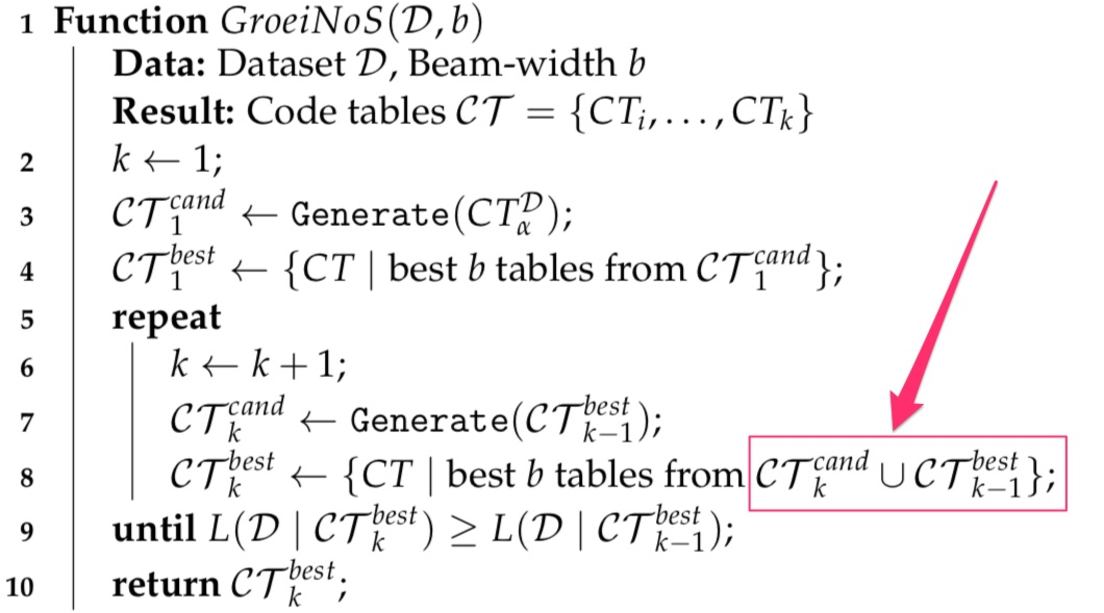
\includegraphics[width=\textwidth]{img/groeinos}
\end{figure}
\end{frame}

\begin{frame}{Clustering Algorithms: Candidate Generation}
\begin{figure}[H]
  \centering
   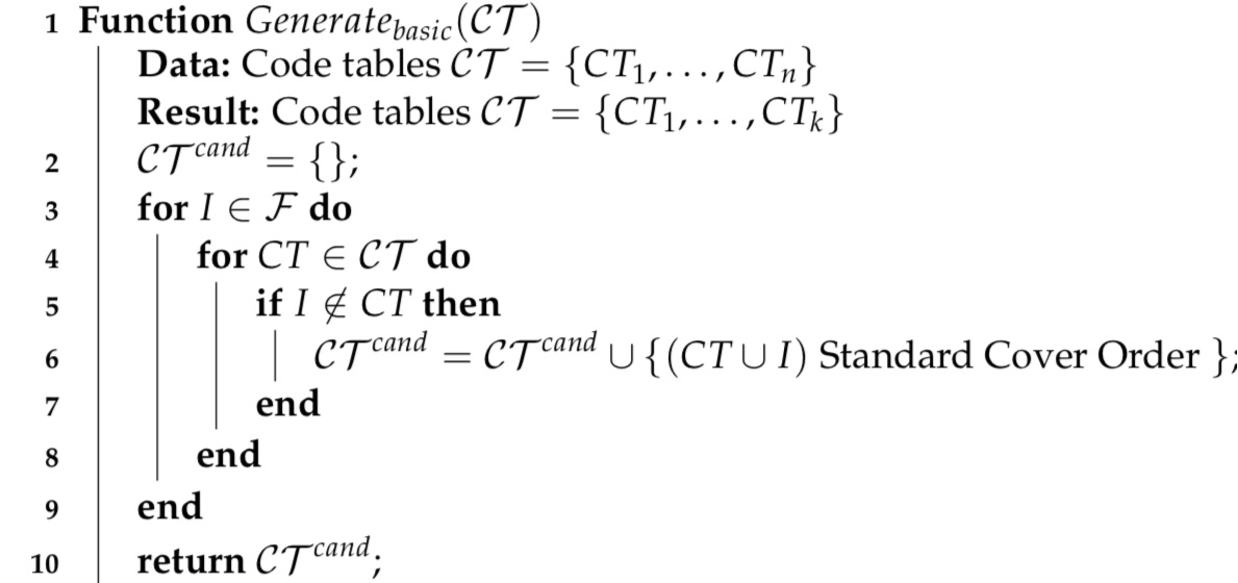
\includegraphics[width=\textwidth]{img/genbasic}
\end{figure}
\end{frame}

\begin{frame}{Clustering Algorithms: Candidate Generation}
\begin{figure}[H]
  \centering
   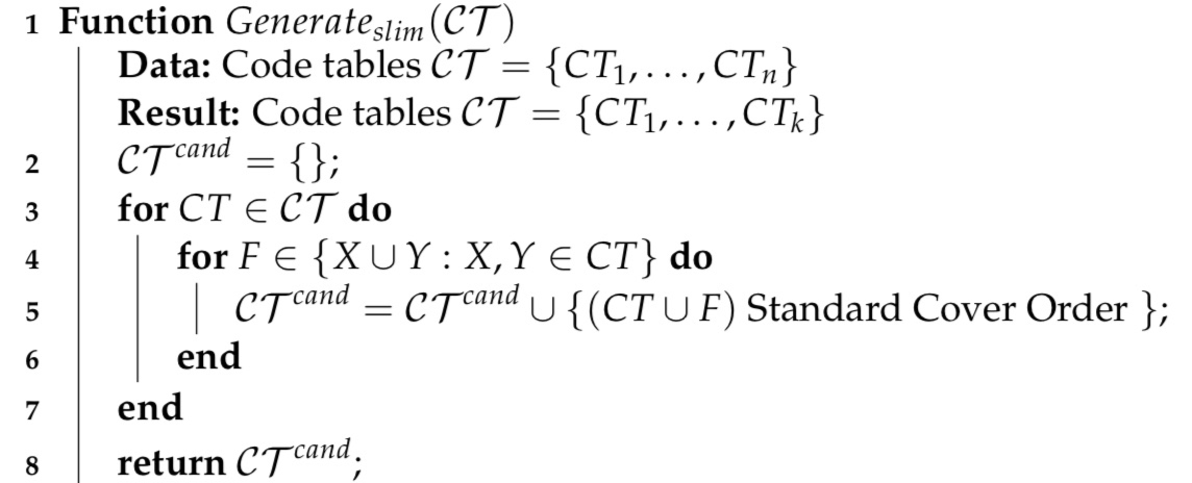
\includegraphics[width=\textwidth]{img/genslim}
\end{figure}
\end{frame}

\section{Experiments}
\begin{frame}{Experiments}
	\begin{itemize}
		\item Setup
		\item Datasets
		\item Compression
		\item Clustering
		\item Classification
		\item Multi-Valued Dependencies
	\end{itemize}
\end{frame}

\begin{frame}{Experiments: Setup}
	\begin{itemize}
		\item Maximum iterations: 250
		\item Cut-off time: 12 hours
		\item All experiments performed on same machine
		\item Default beam-width = 10
		\item Default algorithm: \texttt{GroeiSlimNoS}
	\end{itemize}
\end{frame}

\begin{frame}{Experiments: Datasets}
\begin{table}[H]
\centering
\begin{tabular}{l||l|l|l|l|l}
$\dataset$    & $|\dataset|$  & $|\itemset|$ & $\rho$  & $\theta$    & $|\setitemsets|$  \\ \hline
anneal        & 898           & 71           & 20.1\%  & 100         & $2.55\times10^{4}$ \\
breast        & 699           & 16           & 62.4\%  & 1           & $9.92\times10^{3}$ \\
chess         & 3196          & 75           & 49.3\%  & 2500        & $1.15\times10^{4}$ \\
ionosphere    & 351           & 157          & 22.3\%  & 125         & $1.03\times10^{4}$ \\
iris          & 150           & 19           & 26.3\%  & 1           & $5.43\times10^{3}$ \\
led7          & 3200          & 24           & 33.3\%  & 1           & $1.53\times10^{4}$ \\
mushroom      & 8124          & 119          & 19.3\%  & 2500        & $2.37\times10^{3}$ \\
mammals       & 2183          & 121          & 20.5\%  & 850         & $9.26\times10^{3}$ \\
pageblocks    & 5473          & 44           & 25.0\%  & 1           & $6.36\times10^{4}$ \\
pima          & 768           & 38           & 23.7\%  & 1           & $2.88\times10^{4}$ \\
wine          & 178           & 68           & 20.6\%  & 10          & $8.81\times10^{3}$ \\
wine          & 178           & 68           & 20.6\%  & 20          & $1.45\times10^{3}$ \\
wine          & 178           & 68           & 20.6\%  & 30          & $3.99\times10^{2}$ \\
\end{tabular}
\end{table}
\end{frame}

\begin{frame}{Experiments: Compression}
	\begin{itemize}
		\item General Compression
		\item Runtime
		\item Lowering the support
		\item Beam-width
	\end{itemize}
\end{frame}

\begin{frame}{Experiments: Compression}
\begin{itemize}
	\item Measure the relative compression by the best compressing code table:
			\[ L\% = \frac{L(\dataset,\codetable)}{L(\dataset,\standardtable)} \times 100\% \]
	\item The lower the value of $L\%$, the more structure is captured.
\end{itemize}
\end{frame}

\begin{frame}{Experiments: Compression}
\begin{table}[H]
\resizebox{\textwidth}{!}{%
\begin{tabular}{ll||l|l|l|l|l}
\textbf{$\dataset$} & \textbf{$\theta$} & \texttt{Groei-F} & \texttt{Groei} & \texttt{GroeiNoS} & \texttt{GroeiSlim} & \texttt{GroeiSlimNoS} \\ \hline
anneal                       & 100               & 51,3\%               & 45,2\%         & 45,2\%            & \textbf{43,0\%}             & \textbf{43,0\%}                \\
breast                       & 1                 & 23,2\%               & 16,5\%         & 16,5\%            & \textbf{15,6\%}             & \textbf{15,6\%}                \\
chess                        & 2500              & 65,4\%               & 65,1\%         & 65,1\%            & 65,1\%             & 65,1\%                \\
ionosphere                   & 125               & 78,3\%               & 71,8\%         & 71,8\%            & \textbf{71,1\%}             & \textbf{71,1\%}                \\
iris                         & 1                 & 46,4\%               & 45,5\%         & 45,5\%            & 45,5\%             & 45,5\%                \\
led7                         & 1                 & 39,6\%               & 28,3\%         & 28,3\%            & \textbf{27,4\%}             & \textbf{27,4\%}                \\
mammals                      & 850               & 66,7\%               & 65,3\%         & 65,3\%            & \textbf{65,0\%}             & \textbf{65,0\%}                \\
mushroom                     & 2500              & 66,1\%               & \textbf{65,7\%}         & \textbf{65,7\%}            & 66,2\%             & 66,2\%                \\
pageblocks                   & 1                 & 7,3\%                & 5,0\%          & 5,0\%             & 5,0\%              & 5,0\%                 \\
pima                         & 1                 & 39,1\%               & 33,9\%         & 33,9\%            & \textbf{31,0\%}             & \textbf{31,0\%}                \\
wine                         & 10                & \textbf{71,7\%}               & 72,2\%         & 72,2\%            & 73,0\%             & 73,0\%                \\
wine                         & 20                & \textbf{74,7\%}              & 75,3\%         & 75,3\%            & 75,1\%             & 75,1\%                \\
wine                         & 30                & \textbf{76,8\%}              & 77,5\%         & 77,5\%            & 77,6\%             & 77,6\%               
\end{tabular}
}
\end{table}
\end{frame}

\begin{frame}{Experiments: Compression: Runtime}
\begin{figure}
  \centering
  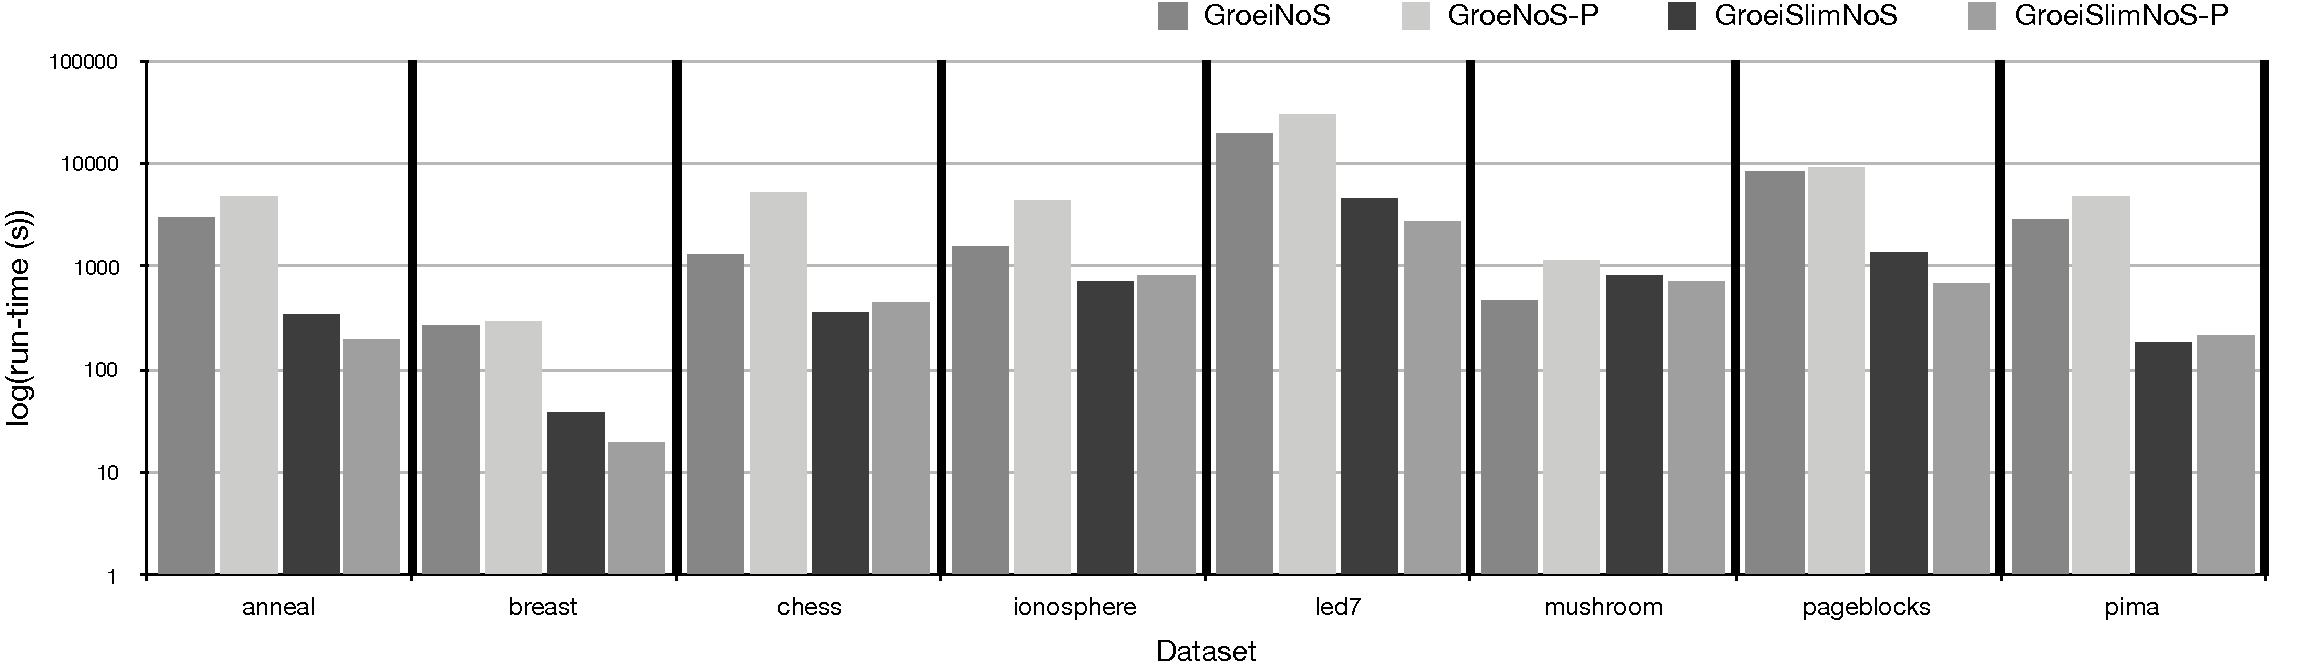
\includegraphics[width=\textwidth]{img/log-run-time}
\end{figure}
\end{frame}


\begin{frame}{Experiments: Compression: Lower Support}
\begin{table}[H]
\centering
\begin{tabular}{l||l|l|l|l|l}
$\dataset$    & $|\dataset|$  & $|\itemset|$ & $\rho$  & $\theta$    & $|\setitemsets|$  \\ \hline             
chess         & 3196          & 75           & 49.3\%  & 500         & $8.46\times10^{9}$ \\
ionosphere    & 351           & 157          & 22.3\%  & 35          & $2.26\times10^{9}$ \\
mushroom      & 8124          & 119          & 19.3\%  & 1           & $1.56\times10^{10}$ \\
mammals       & 2183          & 121          & 20.5\%  & 200         & $9.38\times10^{7}$
\end{tabular}
\end{table}
\end{frame}

\begin{frame}{Experiments: Compression: Lower Support}
\begin{table}[ht]
\centering
\begin{tabular}{ll|ll}
                  &          & \multicolumn{2}{l}{\texttt{GroeiSlimNoS}} \\ \hline
$\dataset$        & $\theta$ & b = 1          & b = 3          \\ \hline
chess*            & 500      & 27,0\%         & 27,0\%         \\
mushroom**        & 1        & 23,5\%         & 23,7\%         \\
ionosphere        & 35       & 56,8\%         & 56,9\%         \\
mammals*          & 200      & 47,0\%         & 46,8\%           
\end{tabular}
\end{table}
 (*) Terminated because of iteration limit. \\
 (**) Terminated because of time limit.
\end{frame}

\begin{frame}{Experiments: Compression: Beam-width}
\begin{figure}[H]
  \centering
   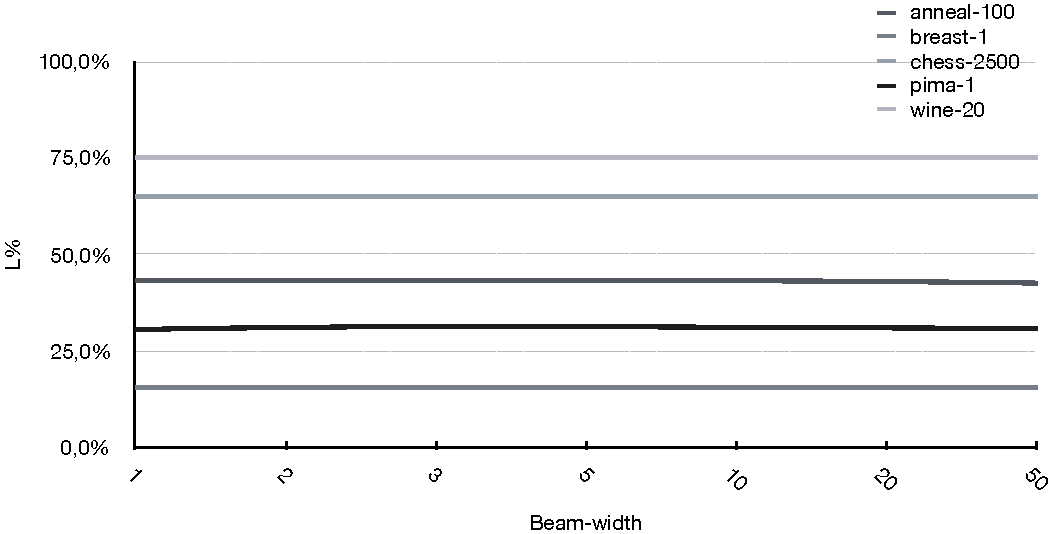
\includegraphics[width=\textwidth]{img/var_bw}
\end{figure}
\end{frame}

\begin{frame}{Experiments: Clustering}
	\begin{itemize}
		\item Entropy of transactions
		\item Dissimilarity between code tables
		\item Probability distribution 
	\end{itemize}
\end{frame}


\begin{frame}{Experiments: Clustering: Entropy}
	\begin{itemize}
		\item Measures the homogeneity of transactions with respect to all clusters.
		\item The higher the entropy, the more uniformly the transaction is compressed by all code tables.
	\end{itemize}
\[E = -\sum\limits_{i=1}^{C} \prob(t \in D_i)\log_{b}\prob(t \in D_i),\]
\end{frame}

\begin{frame}{Experiments: Clustering: Entropy}
\begin{figure}[H]
  \centering
  \begin{subfigure}[b]{0.6\textwidth}
    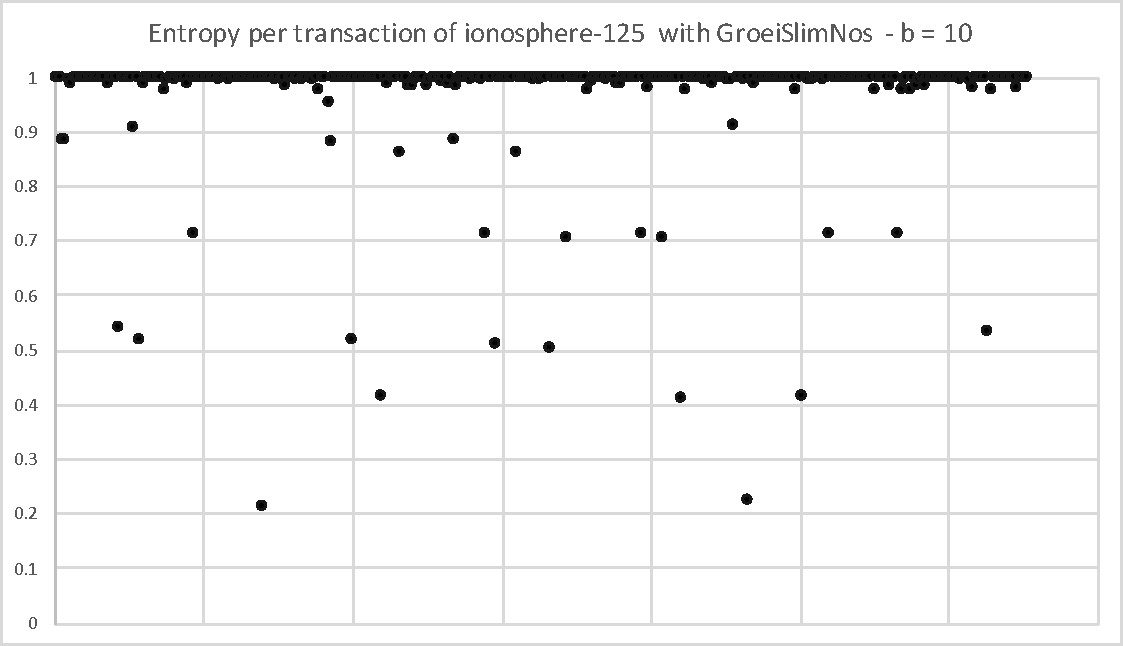
\includegraphics[width=\textwidth]{img/ent-iono-125}
    \caption{ionosphere-125}
  \end{subfigure}

  \begin{subfigure}[b]{0.6\textwidth}
    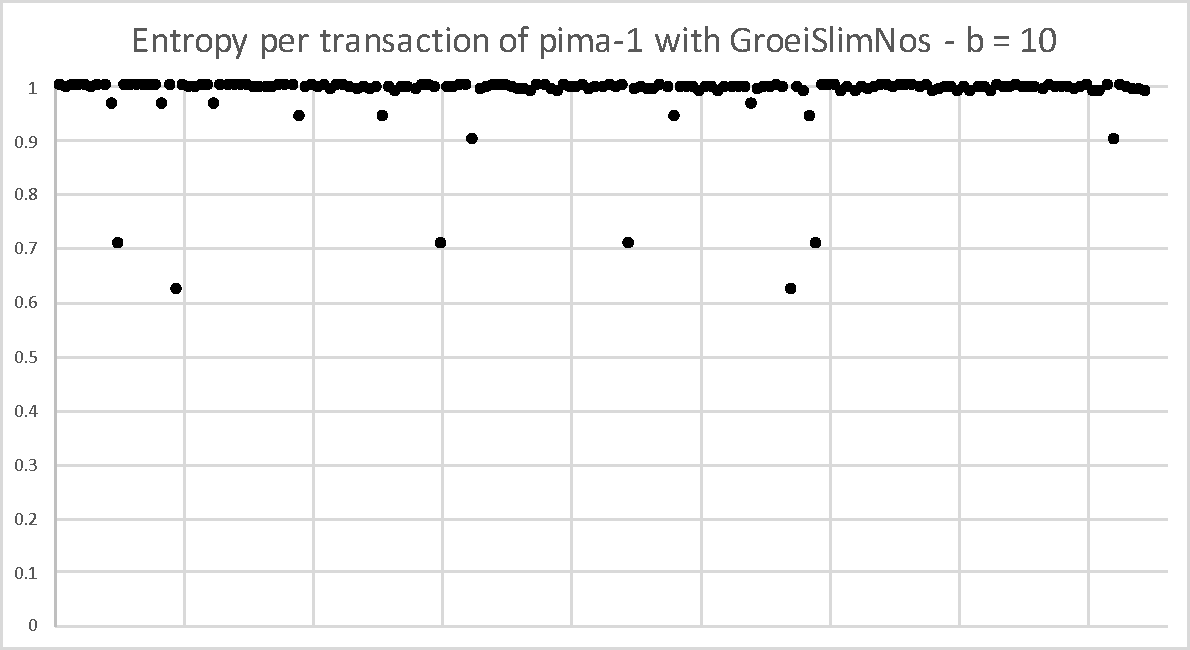
\includegraphics[width=\textwidth]{img/ent-pima-1}
    \caption{pima-1}
  \end{subfigure}
\end{figure}
\end{frame}

\begin{frame}{Experiments: Clustering: Entropy}
\begin{figure}[H]
  \centering
  \begin{subfigure}[b]{0.6\textwidth}
    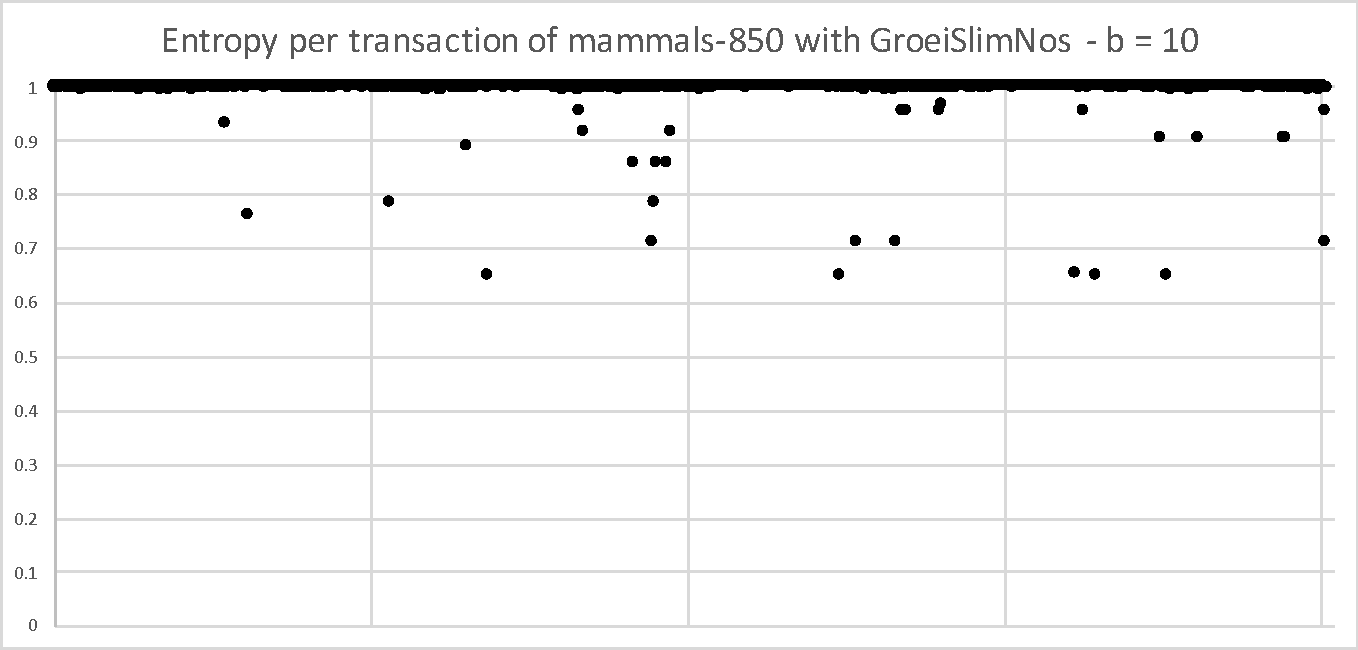
\includegraphics[width=\textwidth]{img/ent-mammals-850}
    \caption{mammals-850}
  \end{subfigure} 

  \begin{subfigure}[b]{0.6\textwidth}
    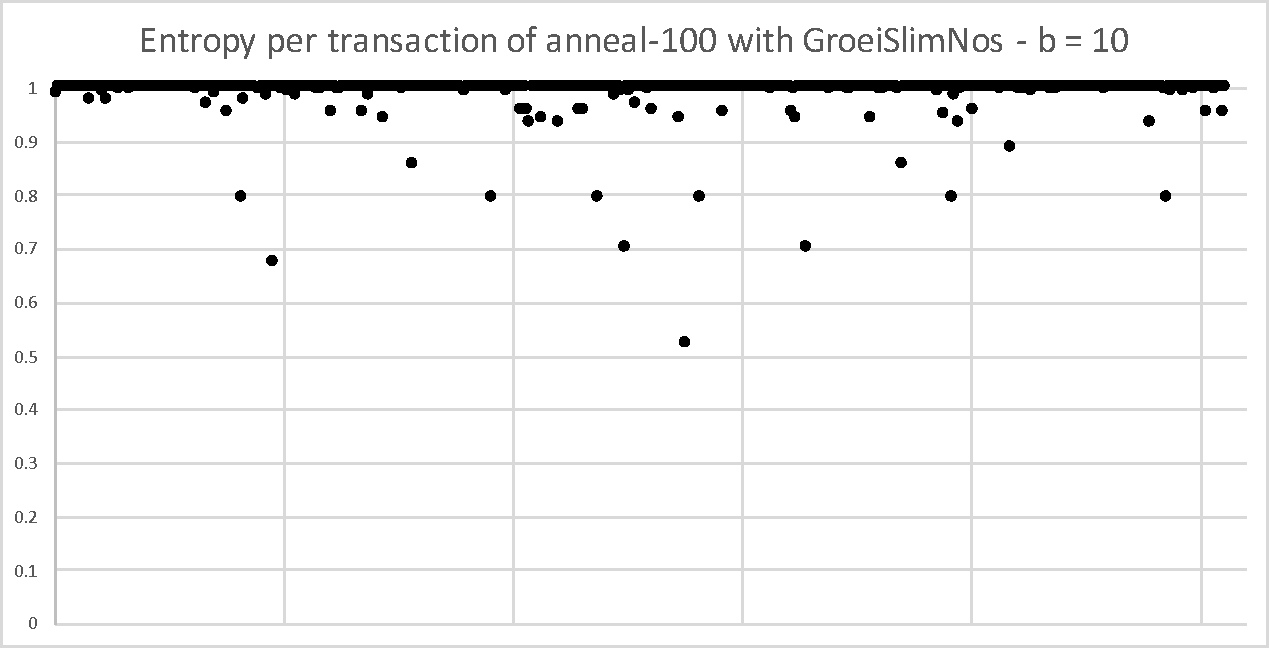
\includegraphics[width=\textwidth]{img/ent-anneal-100}
    \caption{anneal-100}
  \end{subfigure}
\end{figure}
\end{frame}

\begin{frame}{Experiments: Clustering: Dissimilarity}
	\begin{itemize}
		\item Measure the pairwise relative dissimilarity in compressed cluster size.
		\item Code tables are ranked from best compressing to worst compressing.
	\end{itemize}
\[ DS(\codetable_x,\codetable_y,\dataset) = \max\Bigg\{\frac{\codetable_y(\dataset) - \codetable_x(\dataset)}{\codetable_x(\dataset)}, \frac{\codetable_x(\dataset) - \codetable_y(\dataset)}{\codetable_y(\dataset)}\Bigg\} \]
\end{frame}

\begin{frame}{Experiments: Clustering: Dissimilarity}
\begin{figure}
  \centering
  \begin{subfigure}[b]{0.45\textwidth}
    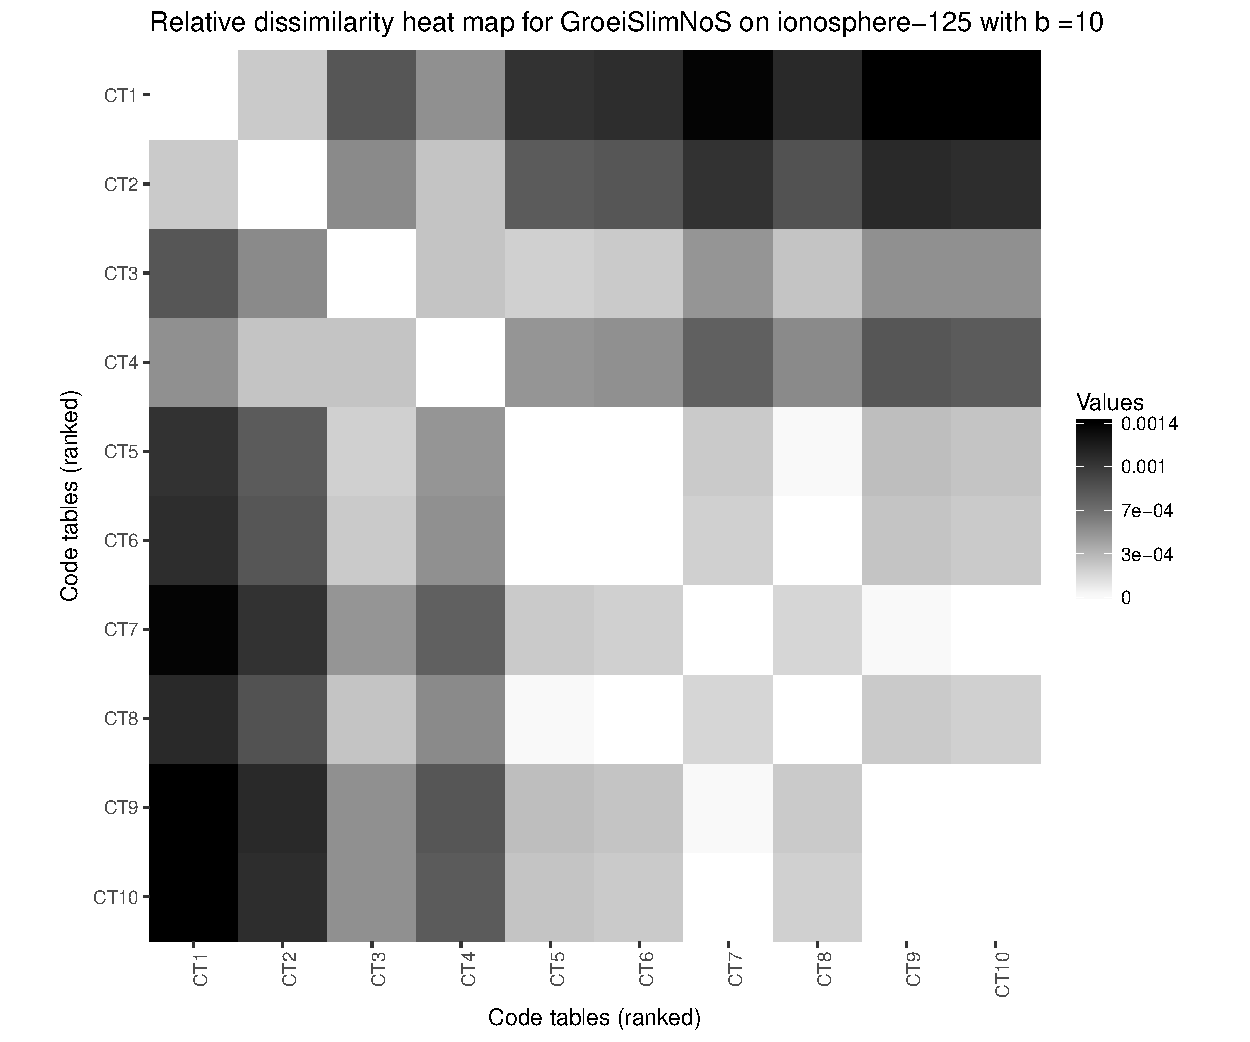
\includegraphics[width=\textwidth]{img/dissim-iono-125}
    \caption{ionosphere-125}
  \end{subfigure}
  \begin{subfigure}[b]{0.45\textwidth}
    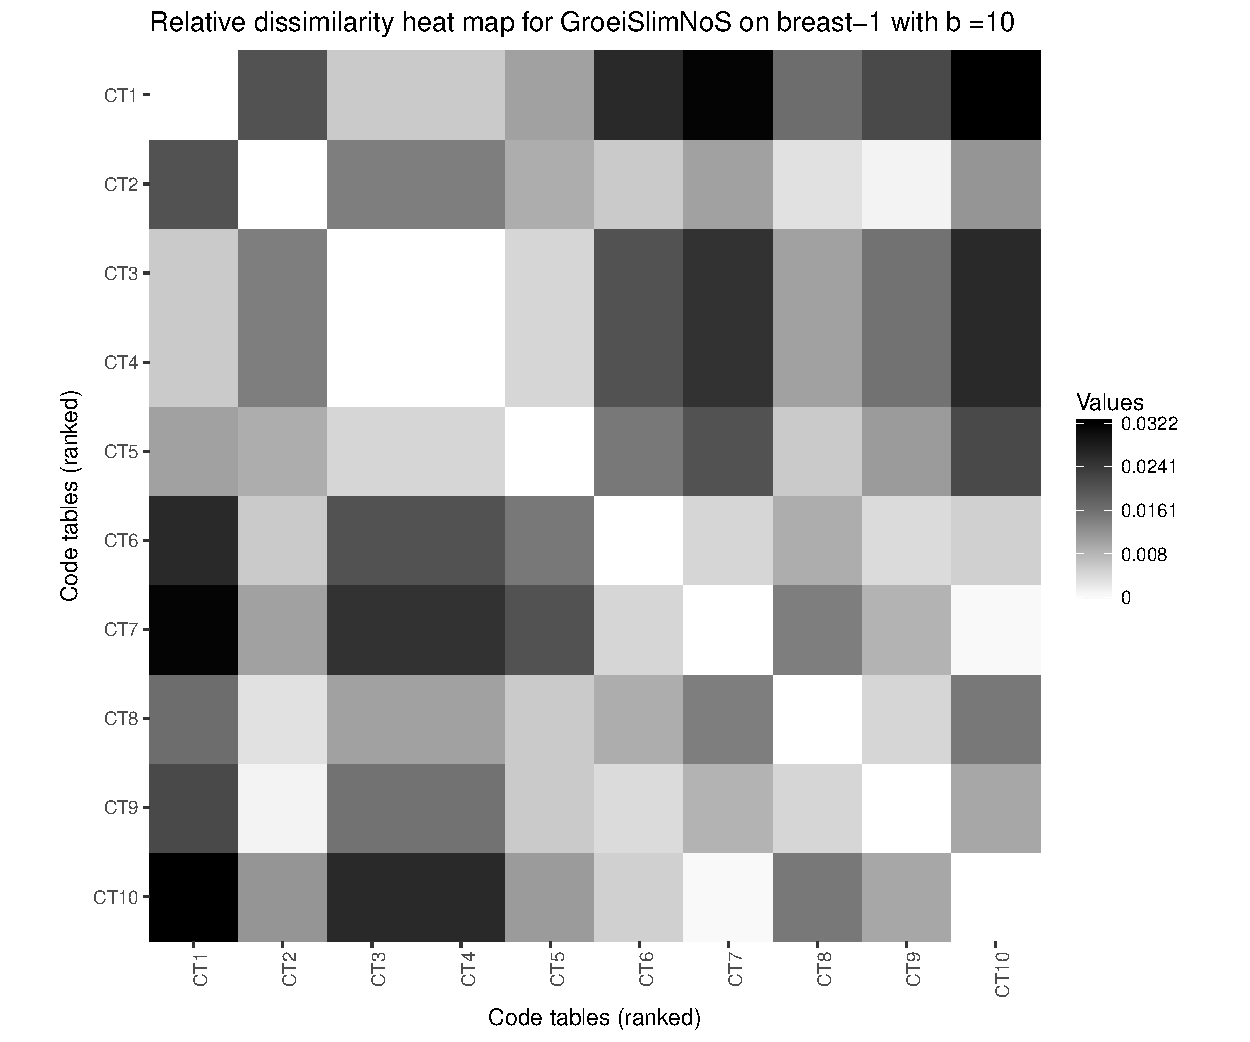
\includegraphics[width=\textwidth]{img/dissim-breast-1}
    \caption{breast-1}
  \end{subfigure} 
\end{figure}
\end{frame}

\begin{frame}{Experiments: Clustering: Dissimilarity}
\begin{figure}
  \centering
  \begin{subfigure}[b]{0.45\textwidth}
    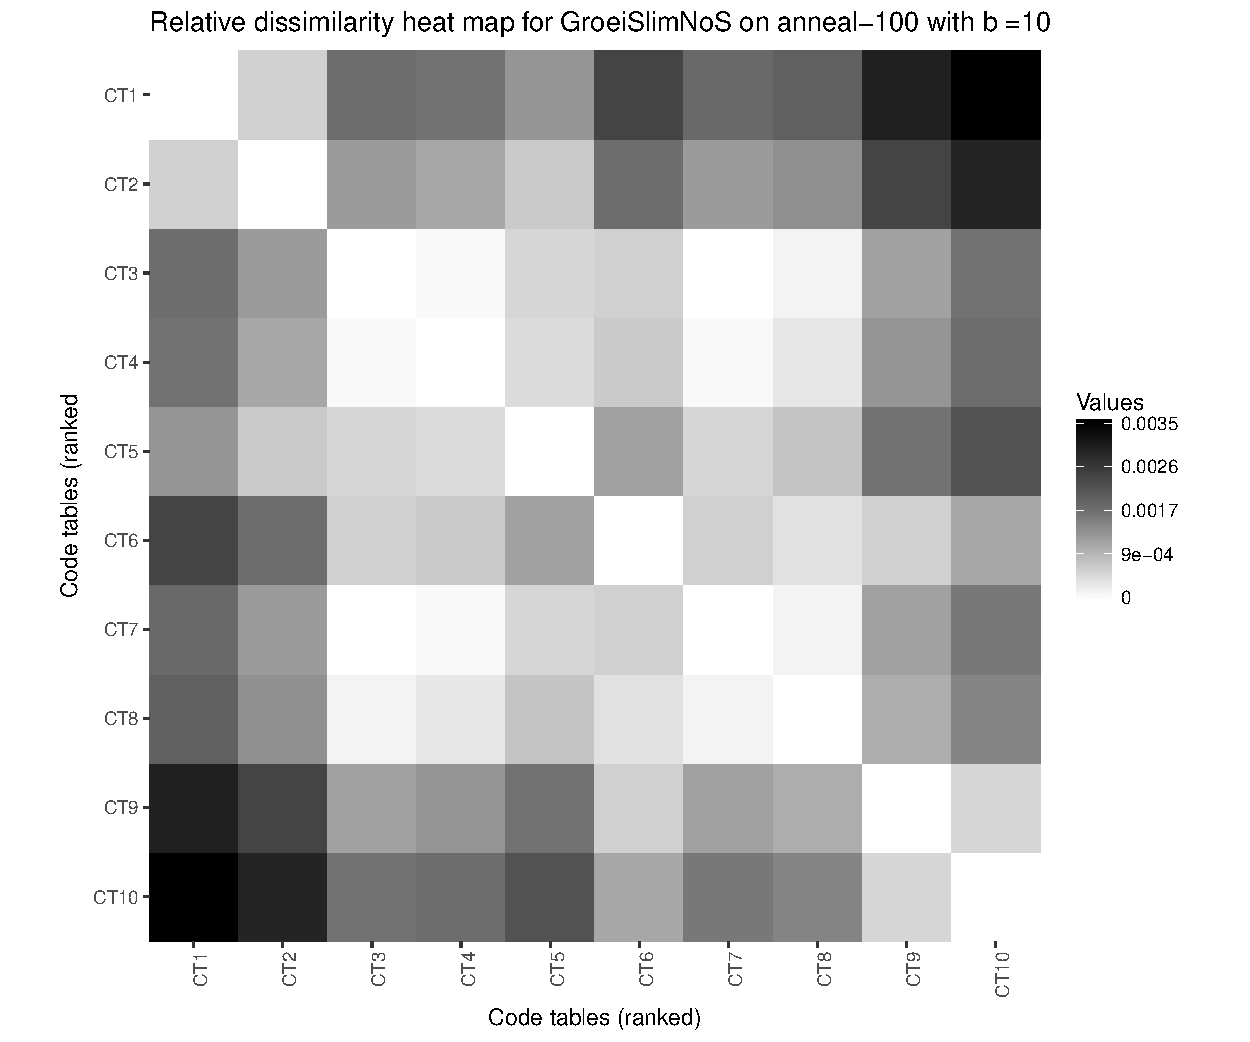
\includegraphics[width=\textwidth]{img/dissim-anneal-100}
    \caption{anneal-100}
  \end{subfigure}
    \begin{subfigure}[b]{0.45\textwidth}
    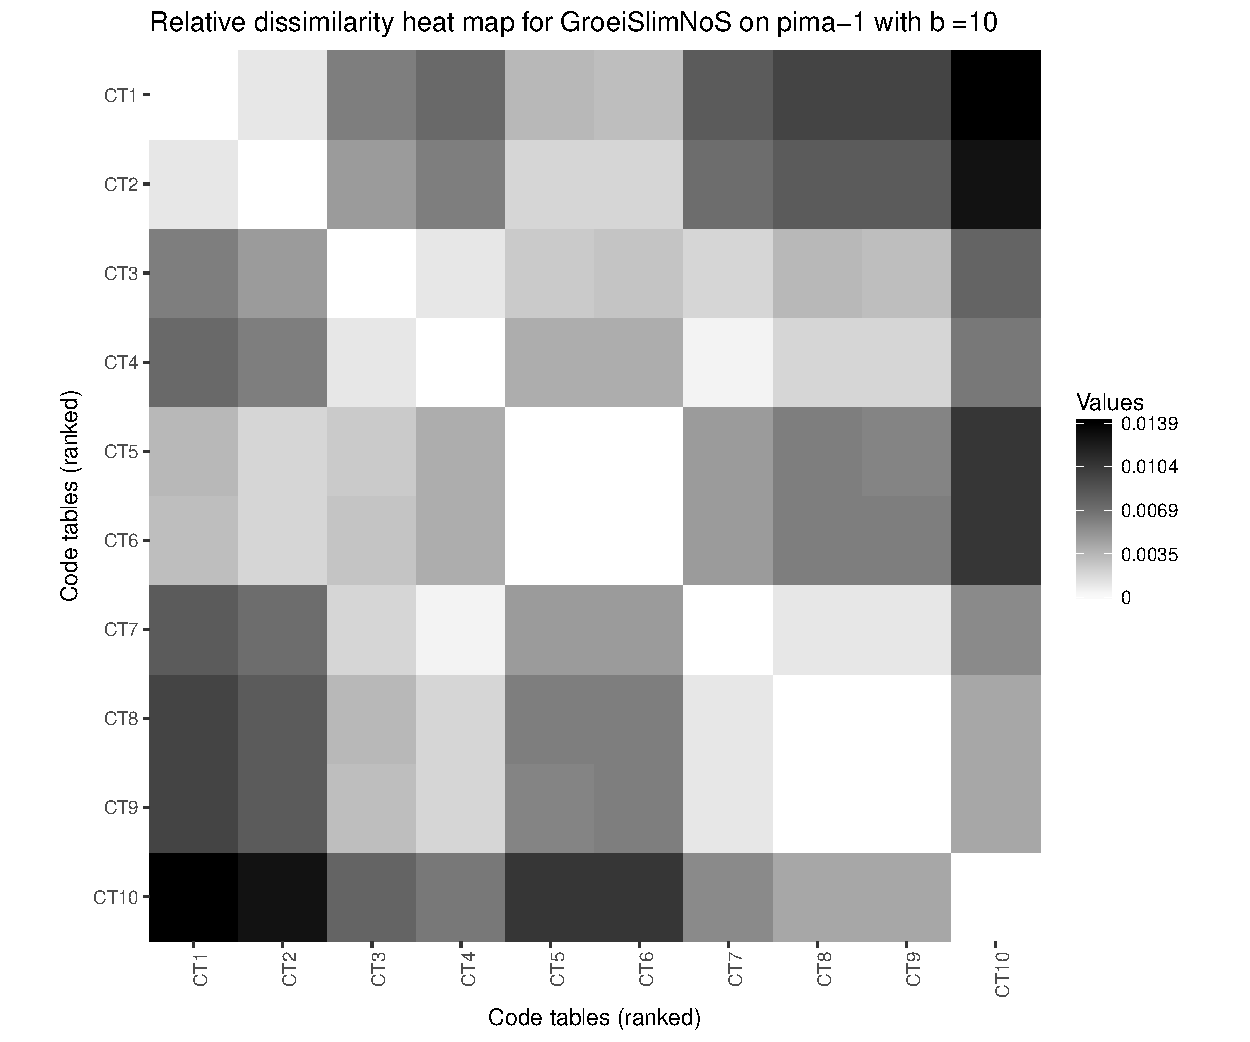
\includegraphics[width=\textwidth]{img/dissim-pima-1}
    \caption{pima-1}
  \end{subfigure}
\end{figure}
\end{frame}

\begin{frame}{Experiments: Clustering: Distribution}
	\begin{itemize}
		\item It also possible to look at a few code tables and the transactions.
		\item This will highlight the differences between the code tables on the level of transactions.
	\end{itemize}
\end{frame}

\begin{frame}{Experiments: Clustering: Distribution: Ionosphere-125}
\begin{figure}
  \centering
  \begin{subfigure}[b]{0.45\textwidth}
    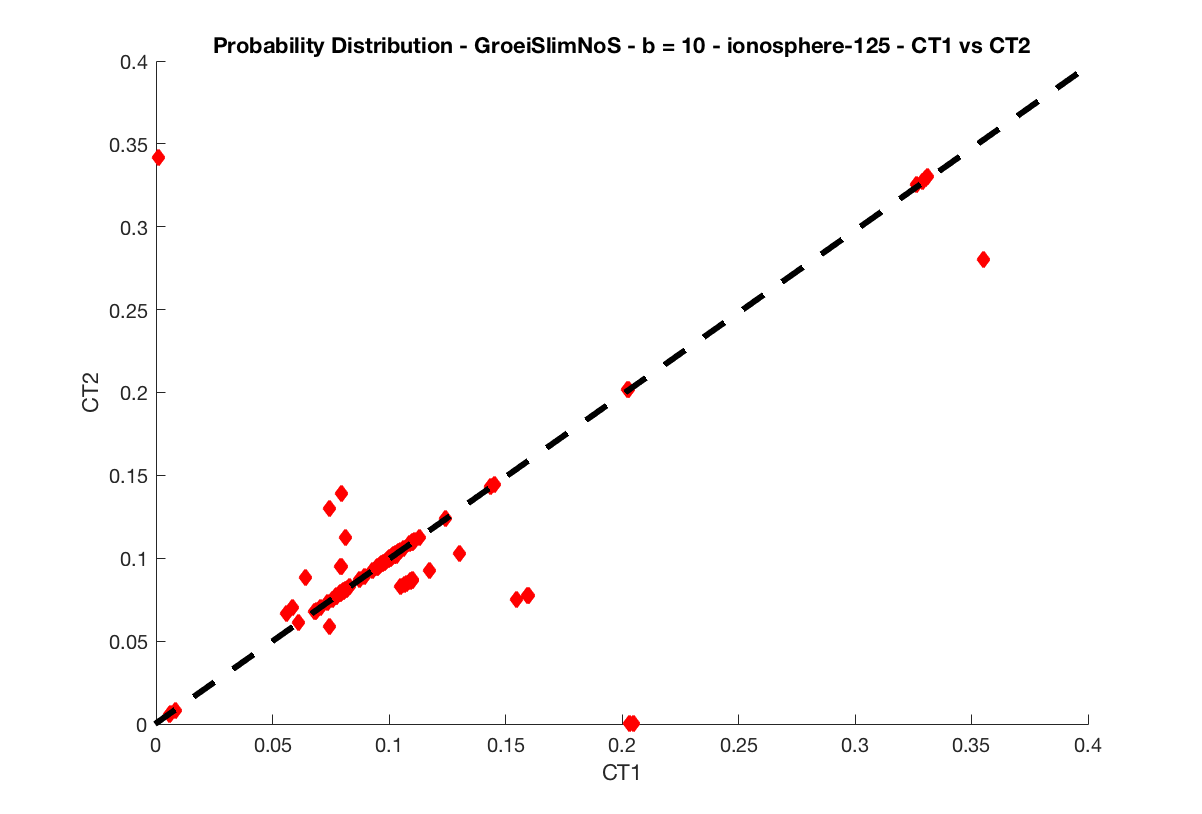
\includegraphics[width=\textwidth]{img/proba-iono125-1-2}
    \caption{$\codetable 1$ versus $\codetable 2$.}
  \end{subfigure}
  \begin{subfigure}[b]{0.45\textwidth}
    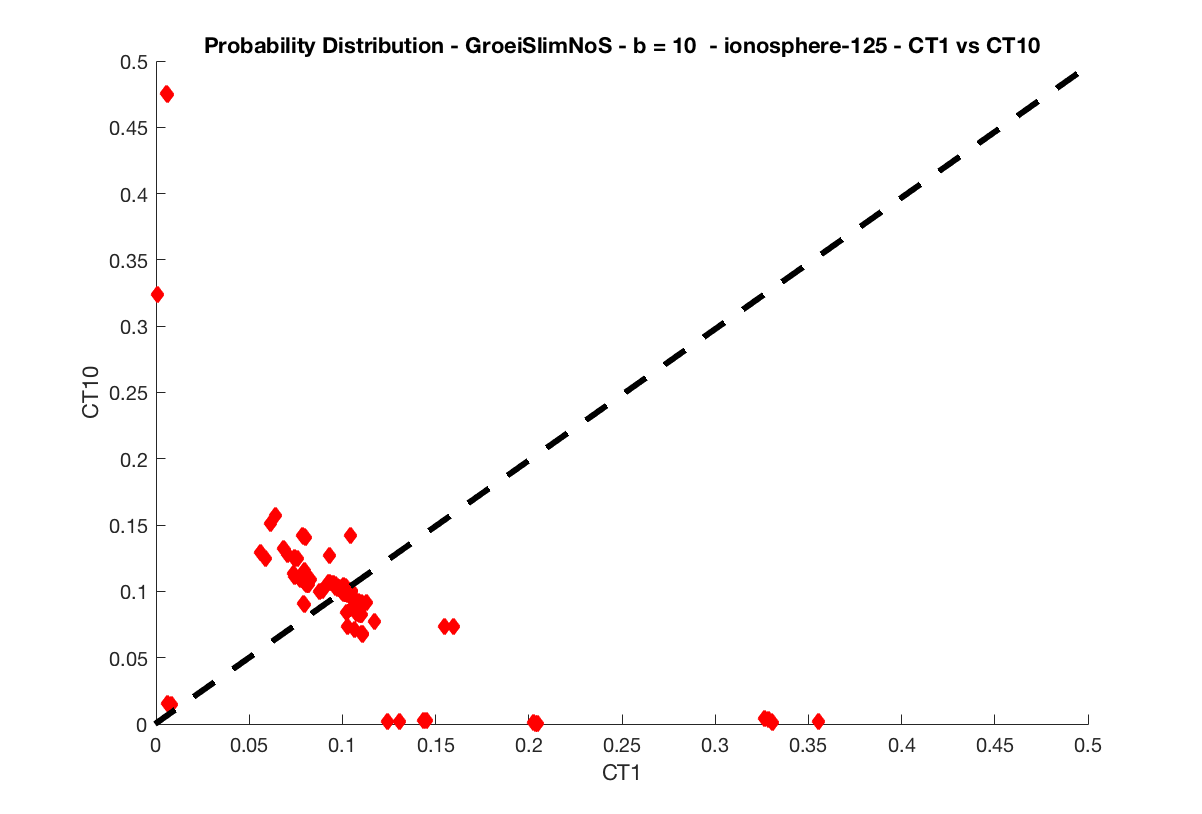
\includegraphics[width=\textwidth]{img/proba-iono125-1-10}
    \caption{$\codetable 1$ versus $\codetable 10$.}
  \end{subfigure} 
\end{figure}
\end{frame}

\begin{frame}{Experiments: Clustering: Distribution: Anneal-100}
\begin{figure}
  \centering
  \begin{subfigure}[b]{0.45\textwidth}
    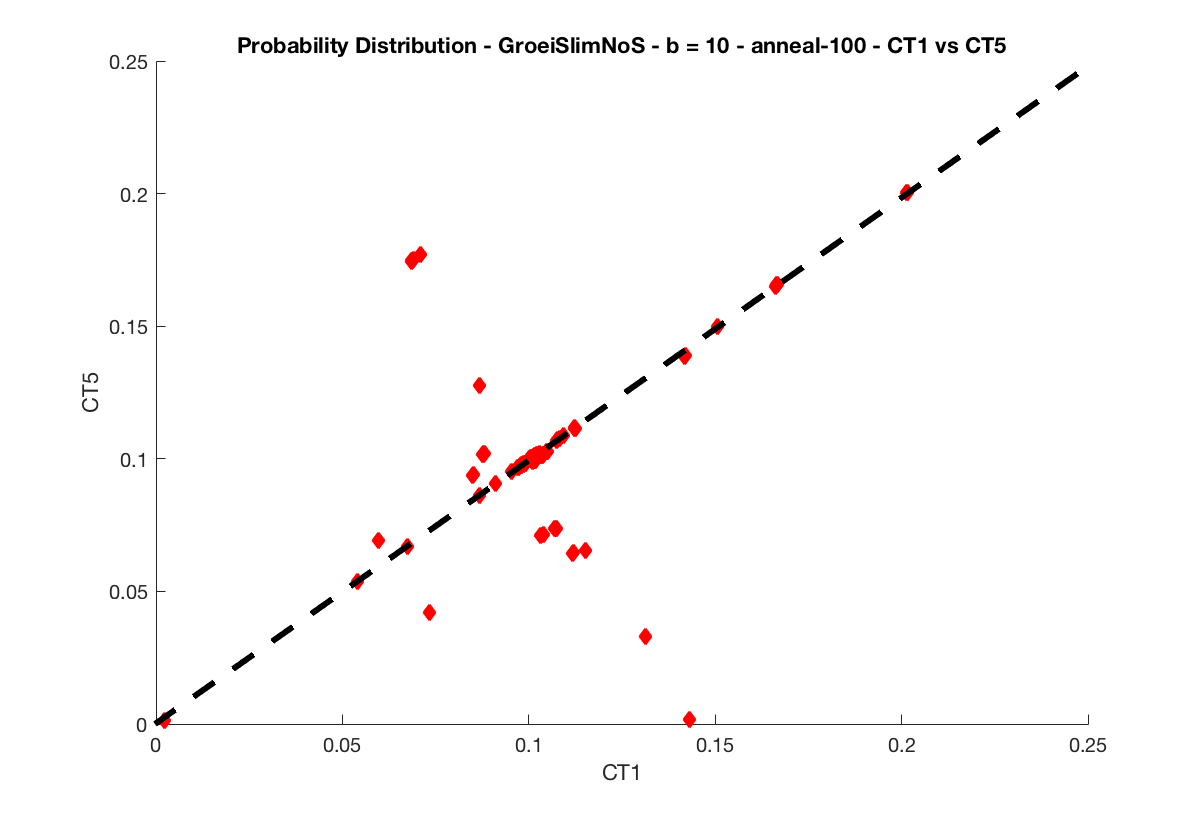
\includegraphics[width=\textwidth]{img/proba-anneal-1-5}
    \caption{$\codetable 1$ versus $\codetable 5$.}
  \end{subfigure}
  \begin{subfigure}[b]{0.45\textwidth}
    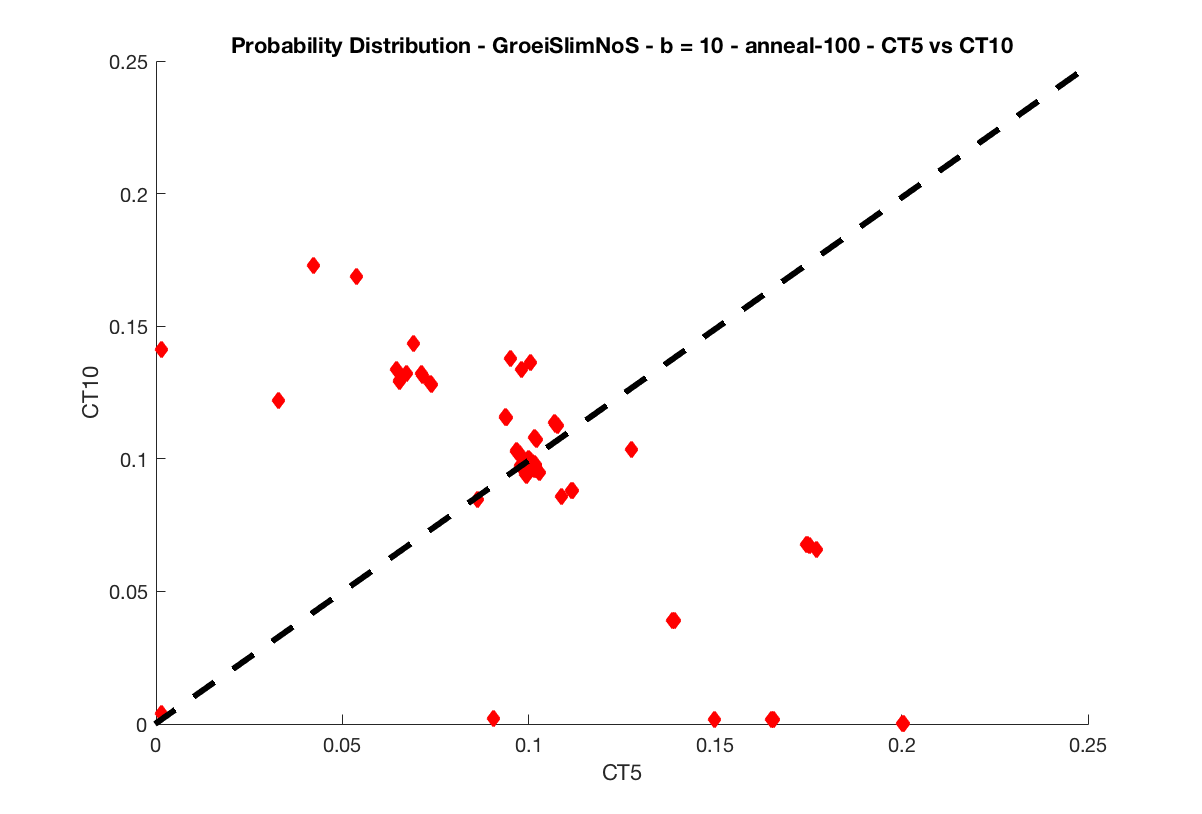
\includegraphics[width=\textwidth]{img/proba-anneal-5-10}
    \caption{$\codetable 5$ versus $\codetable 10$.}
  \end{subfigure} 
\end{figure}
\end{frame}

\begin{frame}{Experiments: Classed Datasets}
	\begin{itemize}
		\item Classification
		\item Purity
	\end{itemize}
\end{frame}

\begin{frame}{Experiments: Classed Datasets: Classification}
\begin{table}[H]
\centering
\begin{tabular}{l|l}
Dataset $\dataset$ & Number of classes $|cl|$ \\ \hline
ionosphere         & 2                        \\
letterrecognition  & 26                       \\
mushroom           & 2                        \\
pendigits          & 10                       \\
wine               & 3                       
\end{tabular}
\end{table}
\end{frame}

\begin{frame}{Experiments: Classed Datasets: Classification}
\begin{itemize}
	\item 10-fold cross validation is used for the experiments.
	\item 1 fold for validation, 9 folds for training.
	\item Training: run the algorithm on each class for each fold.
	\item Assign to the class that compresses the transaction the best.
	\[
\prob(d \in \dataset_i) \propto \frac{1}{\codetable_i(d)}
\]
	\[{C(d) = \argmax\limits_{D_i \in \dataset} \prob(d \in \dataset_i) = \argmax\limits_{D_i \in \dataset} \frac{1}{\codetable_i(d)}}\]
\end{itemize}

\end{frame}

\begin{frame}{Experiments: Classed Datasets: Classification}
	\begin{itemize}
		\item Measure the ratio of cases that have been classified correctly.
		\item Baseline: accuracy when assigning to majority class.
		\[A = \frac{\text{Number of cases classified correctly}}{\text{Total number of cases}}\]
	\end{itemize}
\begin{figure}
  \centering
  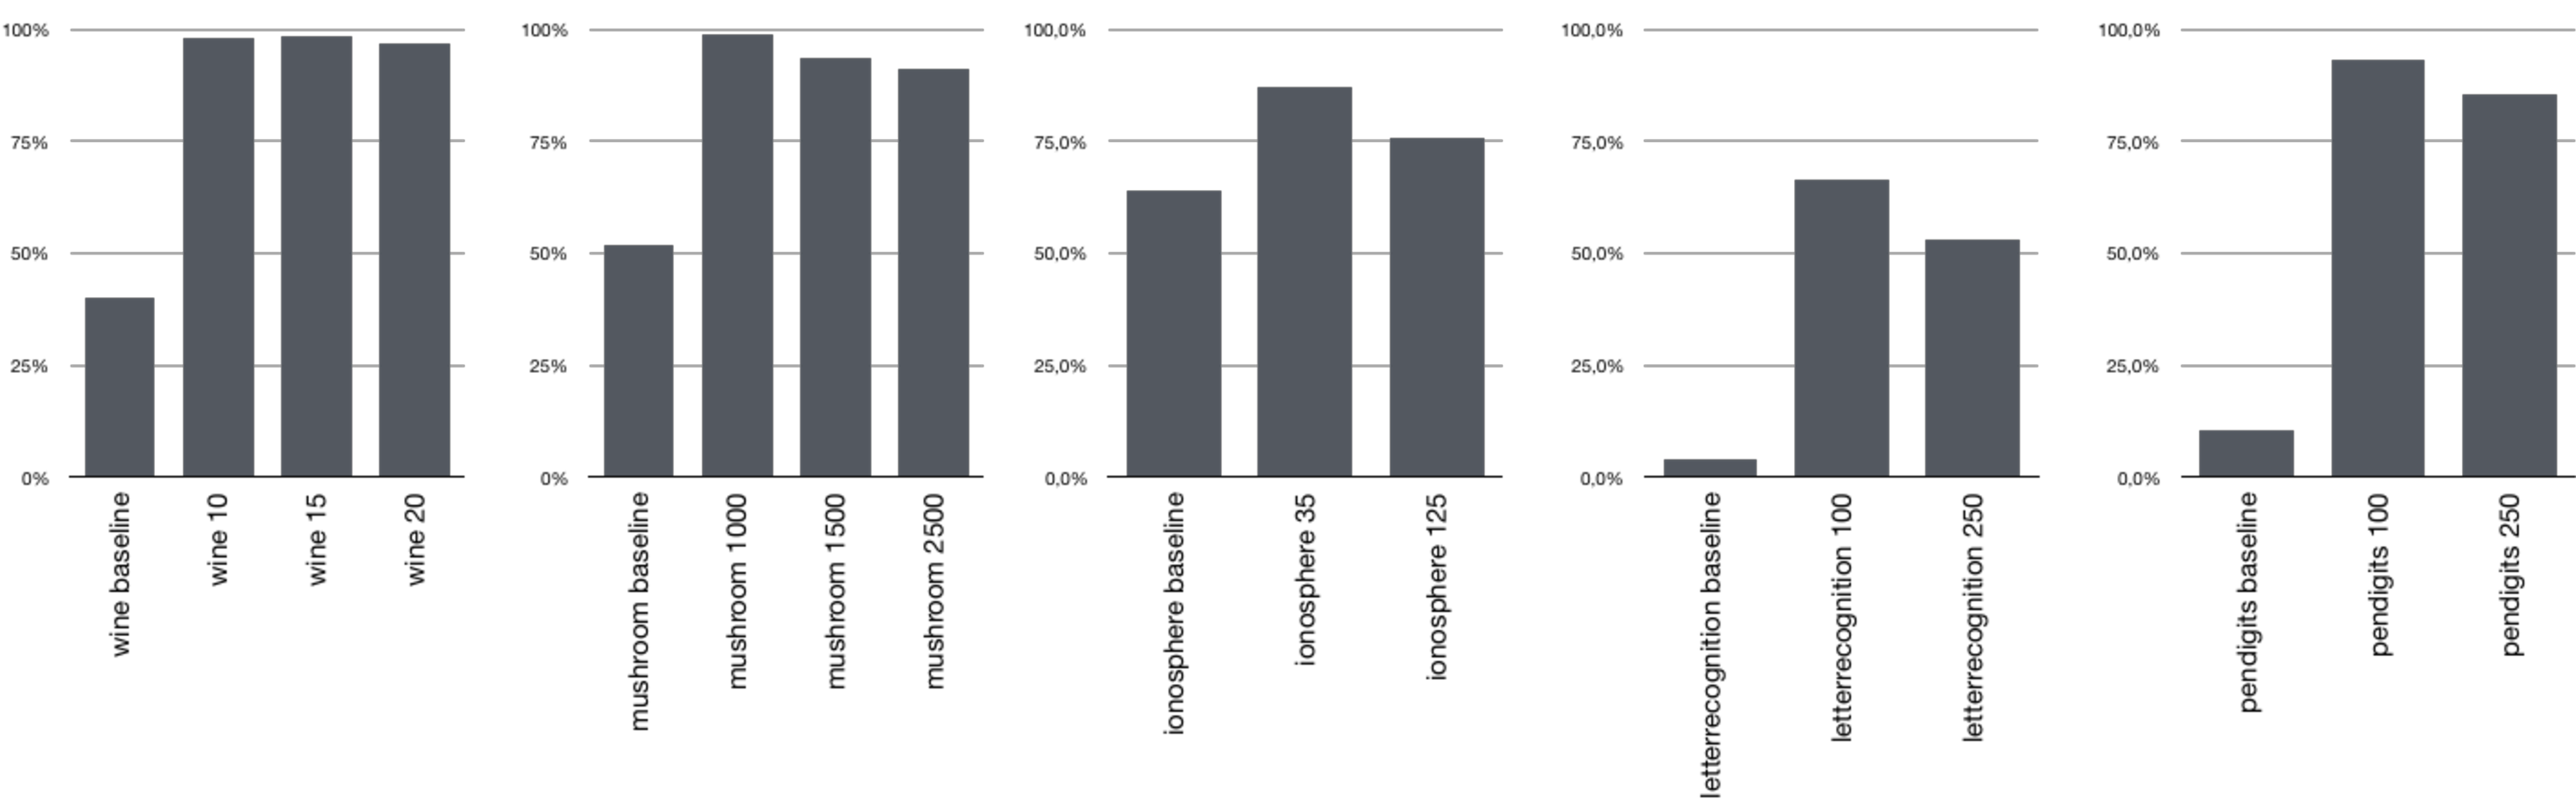
\includegraphics[width=\textwidth]{img/class-all}
\end{figure}
\end{frame}


\begin{frame}{Experiments: Classed Datasets: Purity}
	\begin{itemize}
		\item How well do the obtained clusters characterise the classes? 
		\item Let $\mathscr{D} = \{\dataset_1, \ldots, \dataset_k\}$ the set of clusters, and $\mathscr{C} = \{c_1, \ldots, c_m\}$ denote the set of classes where each class $c_j$ is the set of all cases which belong to $c_j$, then the purity is:
		\[purity(\mathscr{D}, \mathscr{C}) = \frac{1}{N}\sum\limits_{i=1}^{k}\max_j|\dataset_i \cap c_j|\]
		\item Baseline is ratio of classes belonging to the majority class.
		\item beam-width = number of classes
	\end{itemize}
\end{frame}

\begin{frame}{Experiments: Classed Datasets: Purity}

\begin{figure}[H]
  \centering
  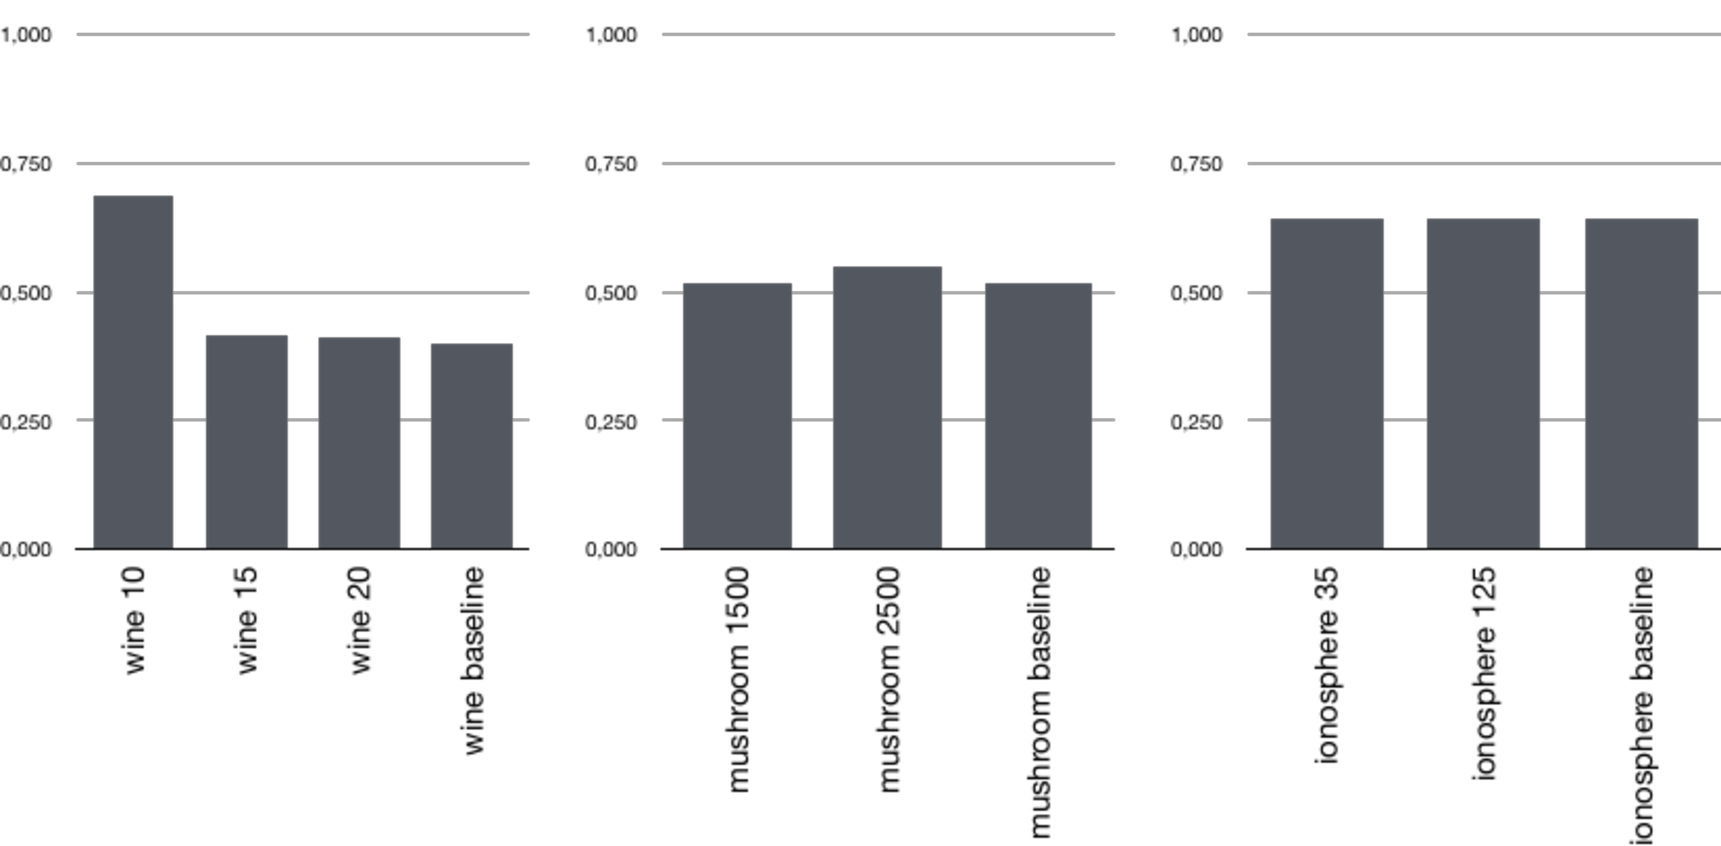
\includegraphics[width=\textwidth]{img/purity}
\end{figure}
\end{frame}

\begin{frame}{Experiments: Multi-Valued Dependencies}
\begin{table}[H]
\centering
\begin{tabular}{l|l}
$(\beta, \gamma, \psi)$ & Number of occurrences  \\ \hline
$(A,J,*)$               & 4                      \\
$(B,K,*)$               & 4                      \\
$(C,K,*)$               & 4                      \\
$(D,L,*)$               & 4                      \\
$(E,M,*)$               & 2                      \\
$(F,K,*)$               & 2                      \\
$(G,J,*)$               & 2                      \\
$(H,L,*)$               & 2                      \\
$(I,J,*)$               & 1                      
\end{tabular}
\end{table}
\end{frame}

\begin{frame}{Experiments: Multi-Valued Dependencies}
\begin{figure}[H]
  \centering
  \includegraphics[width=\textwidth]{img/mvdp123}
\end{figure}
\end{frame}

\section{Discussion}

\begin{frame}{Discussion}
	\begin{itemize}
		\item Compression is on-par or better than \texttt{Groei-F} in most cases.
		\item Big improvement in runtime.
		\item Is able to handle item sets with lower support settings but this can still be improved.
		\item All code tables capture the general patterns
		\item The code tables also capture specific patterns
		\item Classification experiments show that further lowering of the support is required to better capture the structure.
		\item The algorithm is able to identify multi-valued dependencies.
	\end{itemize}
\end{frame}

\section{Conclusion}

\begin{frame}{Conclusion}
	\begin{itemize}
		\item Non-disjoint clustering sheds light on the data from different perspectives.
		\item Both commonalities and differences are identified.
		\item Future work: Further improve candidate generation (USE THE GAIN ORDER!)
	\end{itemize}
\end{frame}

\end{document}